% !TeX spellcheck = it_IT
\section{Wireless Personal Area Network WPAN}

\subsection{ISM Band}

Esistono \textbf{porzioni di banda unlicensed}, ovvero che non necessitano di licenza per essere utilizzate. Sono riservate per usi industriali, scientifici e medici (bande ISM).

Bluetooth, Wi-Fi, apparecchi medici e tutti i dispositivi wireless comunicano sulle stesse bande di frequenze. Trattandosi di uno spazio condiviso, le varie tecnologie devono tollerare interferenze.

\subsection{Pulse Code Modulation PCM}

Si tratta di una \textbf{codifica lossless} per onde. Partendo da un segnale continuo, l'ampiezza della curva viene quantizzata in livelli (intervalli) e viene effettuato un campionamento. La frequenza di campionamento è il doppio della frequenza massima da campionare (teorema del campionamento di Shannon, sezione \ref{par:shannon}).

\begin{center}
	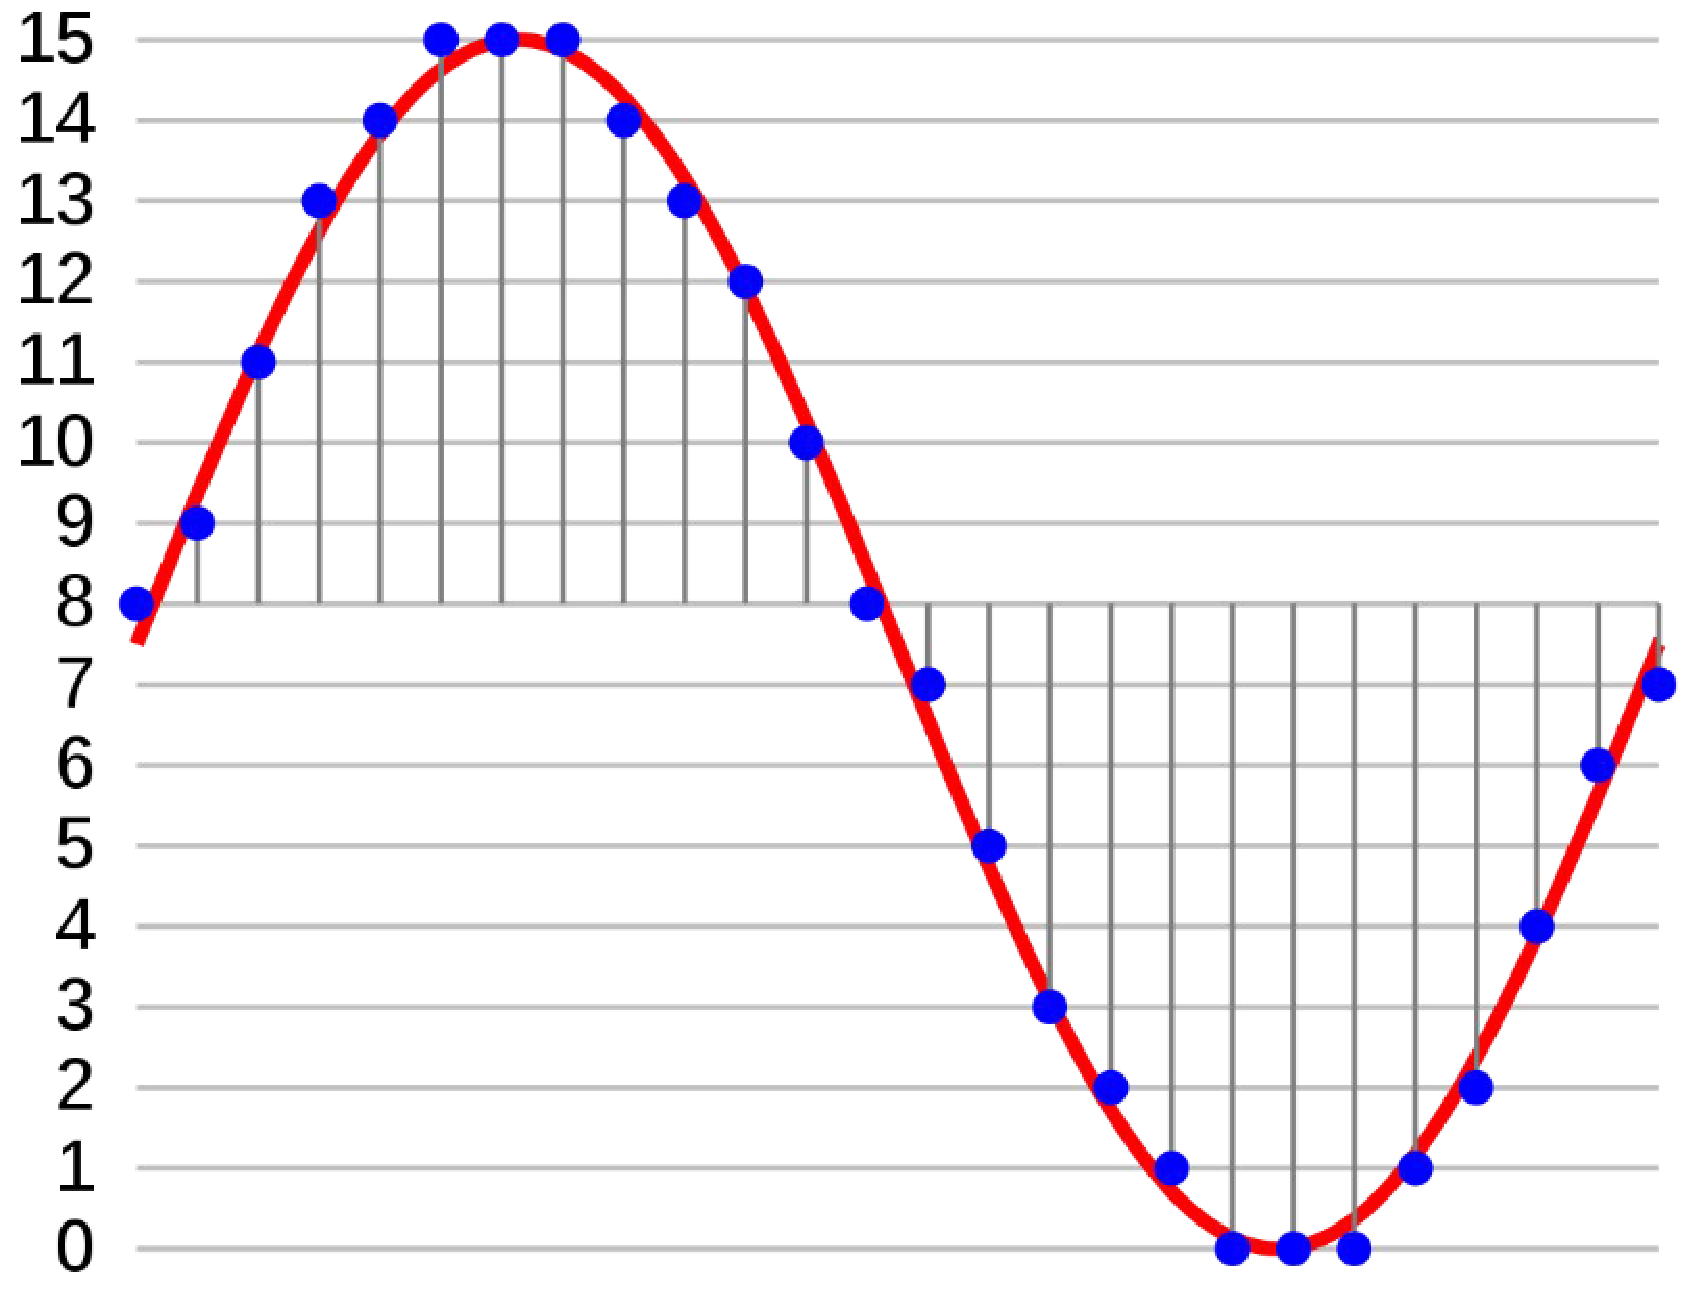
\includegraphics[width=0.7\linewidth]{img/wpan/PCM}
\end{center}

Per la voce telefonica: PCM 8bit $8000Hz$, quindi $64kbps$ (frequenza della voce $300$-$3400Hz$). La musica viene campionata a 24bit, $41/48kHz$.

\subsection{802.15.x}

Lo standard 802.15 comprende un insieme di tecnologie per la \textbf{comunicazione a corto raggio} (\texttt{\url{https://www.ieee802.org/15/}}).

Esempi di tecnologie: 
\begin{itemize}
	\item 802.15.1 Bluetooth

	\item 802.15.2 High-rate WPAN

	\item 802.15.4 Low-rate WPAN (es. Zigbee)

	\item 802.15.5 Mesh Networking (combinazione di High-rate e Low-Rate)

	\item 802.15.6 Body Area Network (BAN) pensato ad esempio per applicazioni in ambito medico

	\item 802.15.7 Visible Light Communication (VLC) (es. Vehicle-to-vehicle communication \& Li-Fi)
\end{itemize}

\subsection{Bluetooth}
Standard 812.15.1. Si compone di reti chiamate \textit{piconet}. All'interno della rete si hanno 
\begin{itemize}
    \item un dispositivo \textbf{master}, controlla la piconet
    
    \item \textbf{uno o più slave}, sotto il controllo del master
\end{itemize}

\textbf{Caratteristiche}: 
\begin{itemize}
	\item Short range (10-50m nei casi d'uso tipici a seconda della classe di potenza del dispositivo, \texttt{\href{https://www.bluetooth.com/learn-about-bluetooth/key-attributes/range/\#estimator}{Bluetooth range estimator}})
	
    \item Usa la banda ISM $2.4GHz$
	
    \item Data Rate: $2.1 Mbps$-$24Mbps$
\end{itemize}

\paragraph{Utilizzi:}
\begin{itemize}
	\item punto di accesso per dati e voce

	\item sostituzione di cavi (periferiche wireless)

	\item comunicazione ad hoc con altri dispositivi Bluetooth
\end{itemize}

\subsubsection{Architettura dei protocolli} 

\begin{center}
	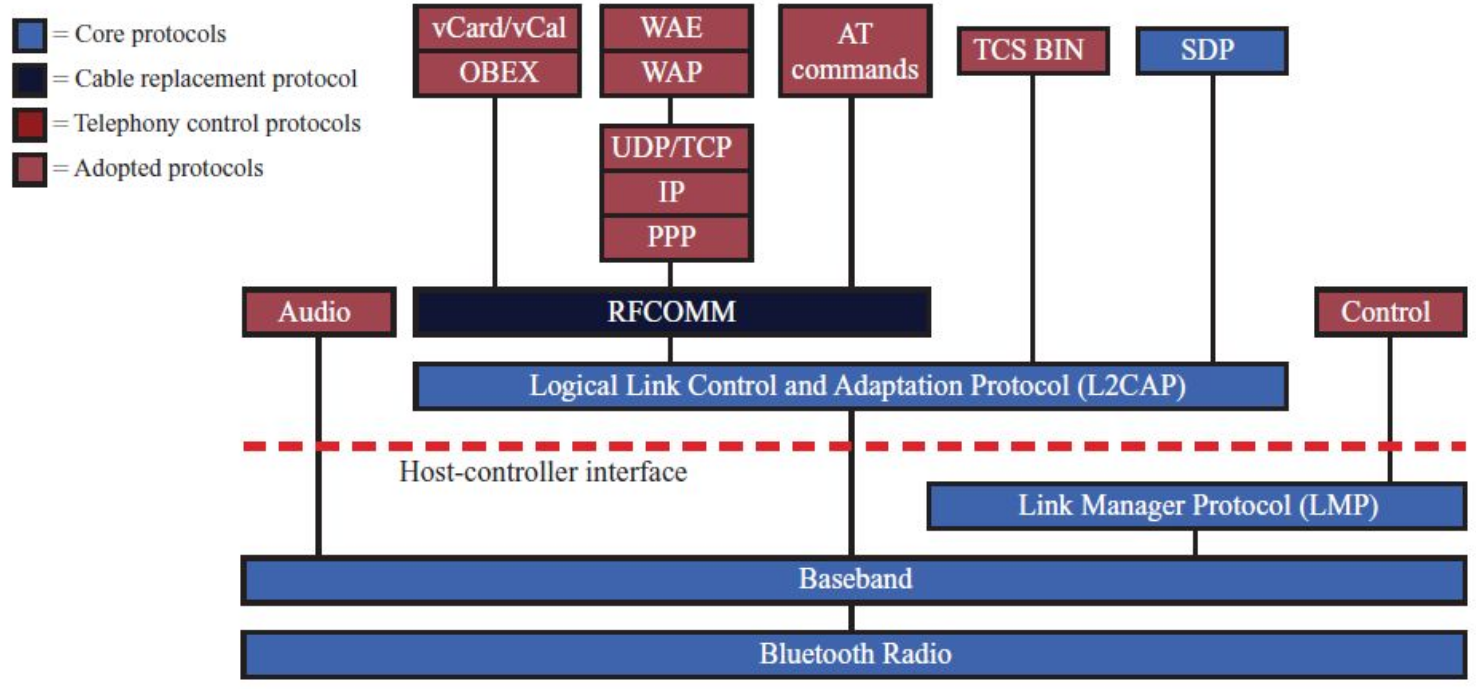
\includegraphics[width=0.95\linewidth]{img/wpan/archbt}
\end{center}

In blu sono i "\textit{core protocols}", ovvero le componenti necessariamente presenti all'interno di tutti i dispositivi Bluetooth. Gli altri (rossi e blu scuro) sono implementati solo se il dispositivo ne necessita, quindi in base al caso d'uso.

\paragraph{Bluetooth Radio:} La parte di livello fisico, specifica l'interfaccia radio: 
\begin{itemize}
	\item radio frequenze, quali frequenze utilizzare
	
    \item gestisce il frequency hopping
	
    \item decide lo schema di modulazioni in base al canale
	
    \item determina la potenza di trasmissione
\end{itemize}

\paragraph{Baseband:} Il livello di Baseband si occupa di 
\begin{itemize}
	\item stabilire la connessione con la piconet

	\item gestire l'indirizzamento

	\item formattazione dei pacchetti (frame)

	\item gestire le tempistiche di comunicazione (Time Division Duplex TDD e Time Division Multiple Access TDMA)

	\item gestire la potenza di trasmissione (passa le indicazioni a livello radio)
\end{itemize}

\paragraph{Link Manager Protocol LMP:} Fa da "manager" del collegamento. Si occupa di:
\begin{itemize}
	\item configurare i collegamenti tra dispositivi

	\item gestire i collegamenti attivi

	\item gestire funzionalità di sicurezza e cifratura
\end{itemize}

Si tratta di un protocollo di controllo, non passano dati, gestisce solamente il collegamento per i livelli sottostanti.

\paragraph{Logical Link Control and Adaptation Protocol (L2CAP):} I livelli precedenti erano presenti fisicamente sul chip Bluetooth, da questo in su sono implementati a livello software. 

L2CAP si occupa di:
\begin{itemize}
	\item adattare i protocolli di livello superiore al livello baseband
	
    \item astrarre le feature esposte dai livelli inferiori per i servizi a livelli superiori, \textit{Connectionless} e \textit{Connection-oriented}
\end{itemize}

\paragraph{Service Discovery Protocol SDP:} Gestisce le informazioni del dispositivo. Permette di comunicare
\begin{itemize}
	\item servizi disponibili sul dispositivo
    
	\item caratteristiche sul dispositivi
\end{itemize}

Lo stile dell'architettura è client-server: prevede interrogazioni richiesta-risposta per stabilire connessioni tra dispositivi Bluetooth.

\paragraph{Radio Frequency Communication RFCOMM:} Astrae il livello di Bluetooth, permette di "\textit{simulare un cavo}". Simula una comunicazione seriale e permette la trasmissione di dati tra dispositivi Bluetooth.

\paragraph{Livelli superiori:} I livelli in rosso sono protocolli "\textit{già esistenti}", ciascun dispositivo può implementare tutti o parte di questi protocolli in base all'uso. 

I livelli inferiori sono quelli che permettono la comunicazione a livello fisico.

\paragraph{Profili:} Per avere determinate funzionalità un dispositivo deve seguire dei "profili". 

Esempi di profili:
\begin{center}
	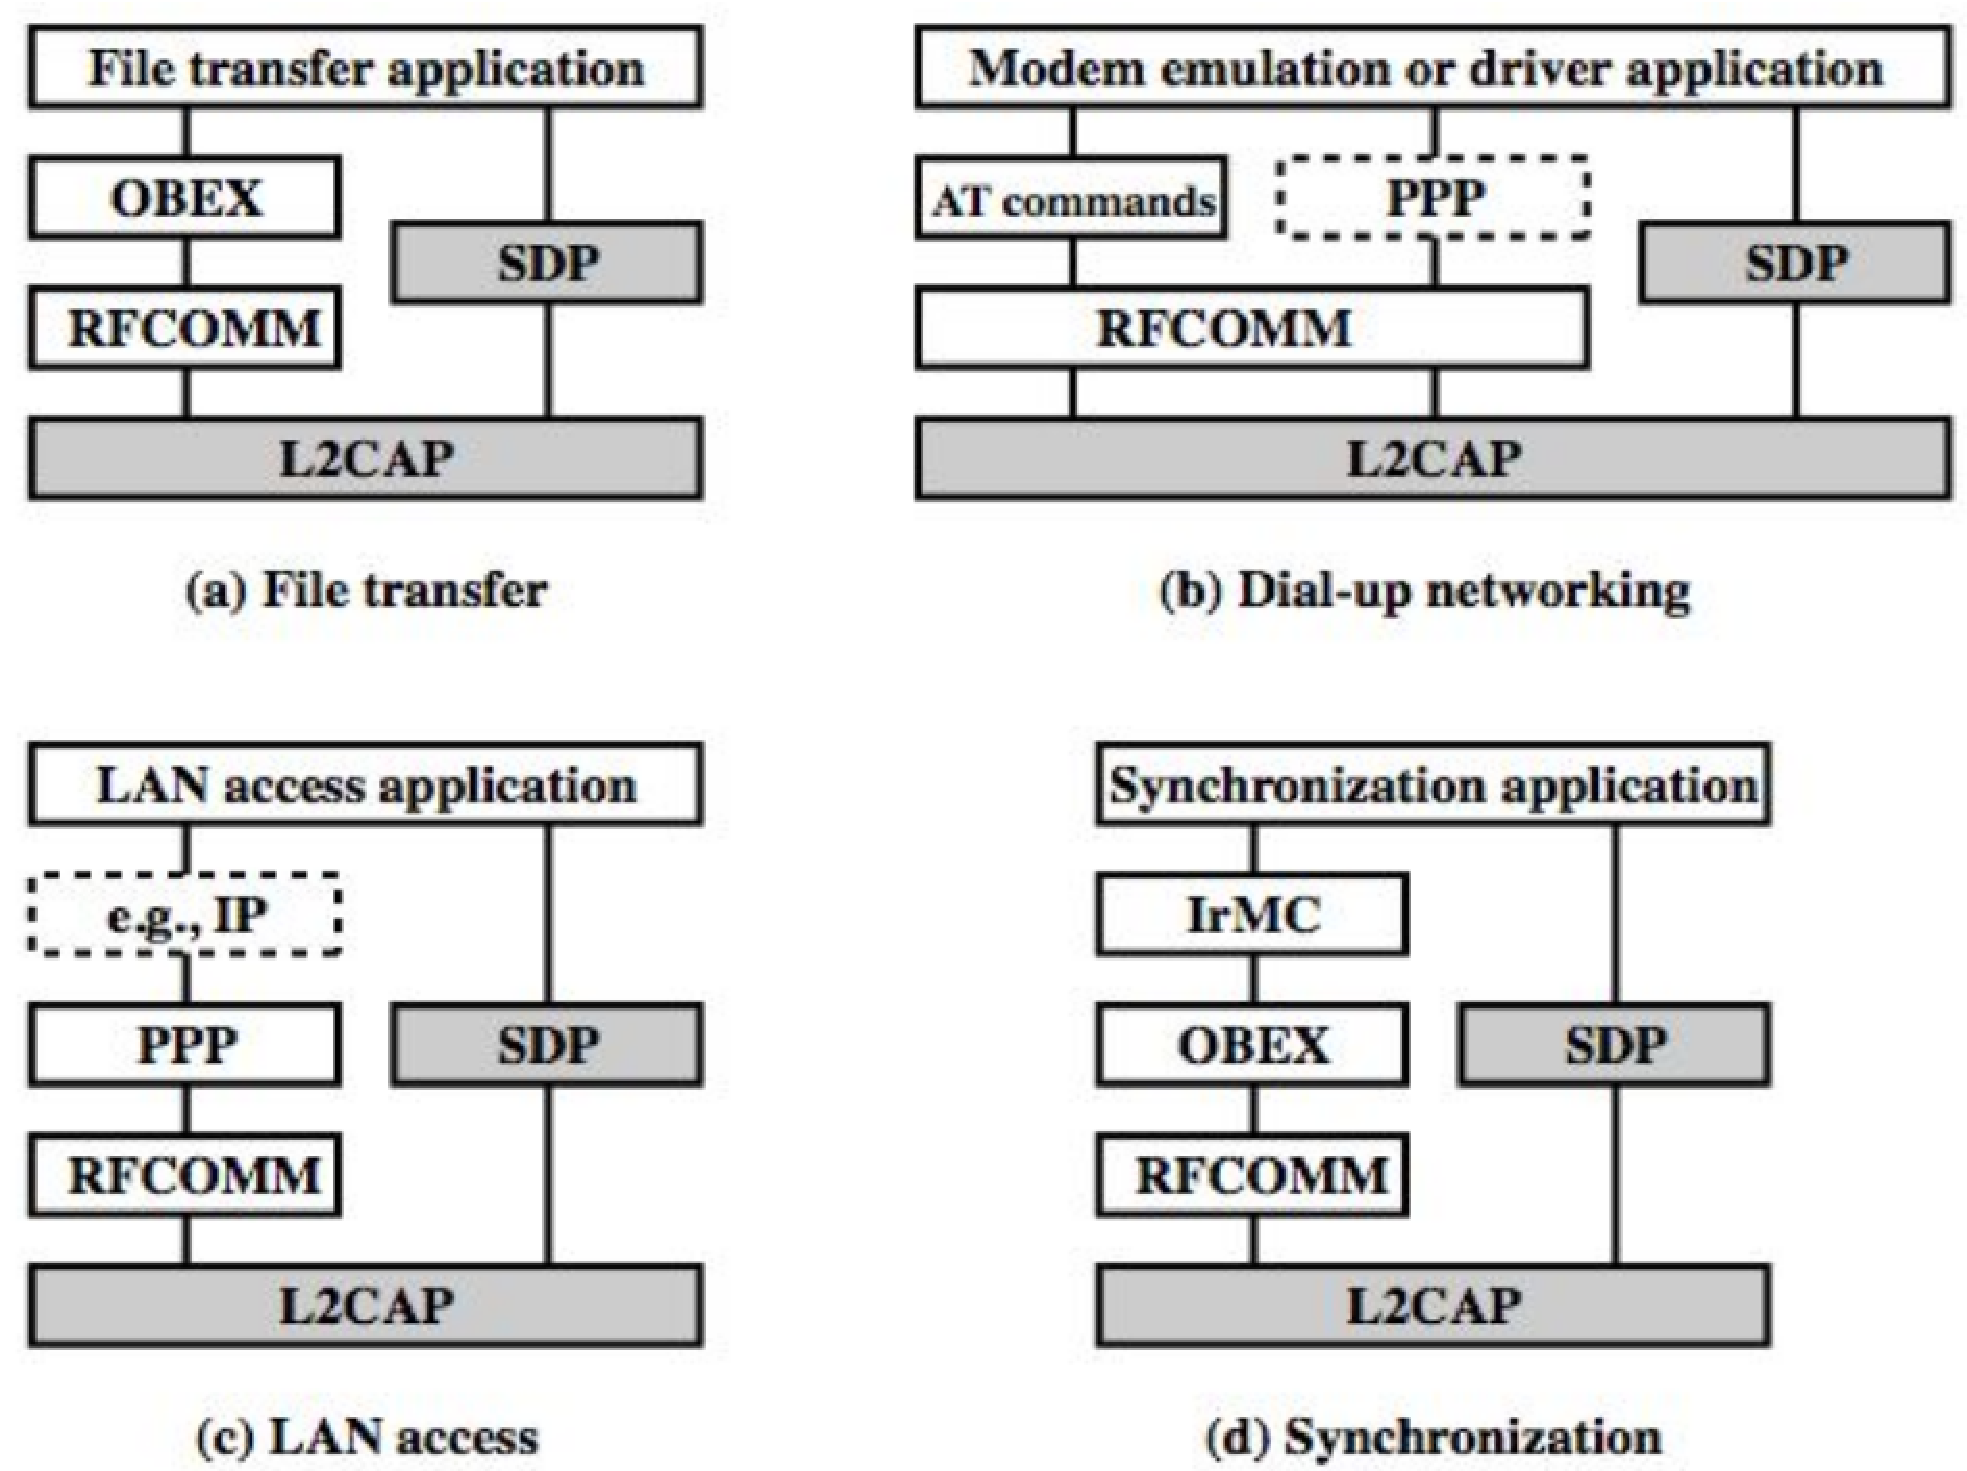
\includegraphics[width=0.8\linewidth]{img/wpan/profiles}
\end{center}

Questi sono standard, un dispositivo deve aderire a uno o più profili (annunciati dal SDP) per avere il relativo utilizzo.

\subsubsection{Piconet \& Scatternet}

\paragraph{Piconet:} Una piconet è composta da un \textbf{master} e
\begin{itemize}
	\item \textbf{Active Slave (AS)}: membro attivo delle piconet, con un indirizzo Active Member Address (AMA) su 3 bit assegnato dal master (0 è il master, quindi 7 dispositivi al massimo)
	
    \item \textbf{Parked Slave (PS)}: membro della piconet ma temporaneamente disattivato, non possono comunicare attivamente ma solo ogni tanto tramite il Parked Member Address (PMA), 8 bit (0 è il master); un parked può tornare attivo solo se "c'è spazio"
	
    \item \textbf{Standby Slave (SS)}: non sconosciuti ma scollegati; non hanno indirizzi e possono quindi essere infiniti
\end{itemize}
\begin{center}
	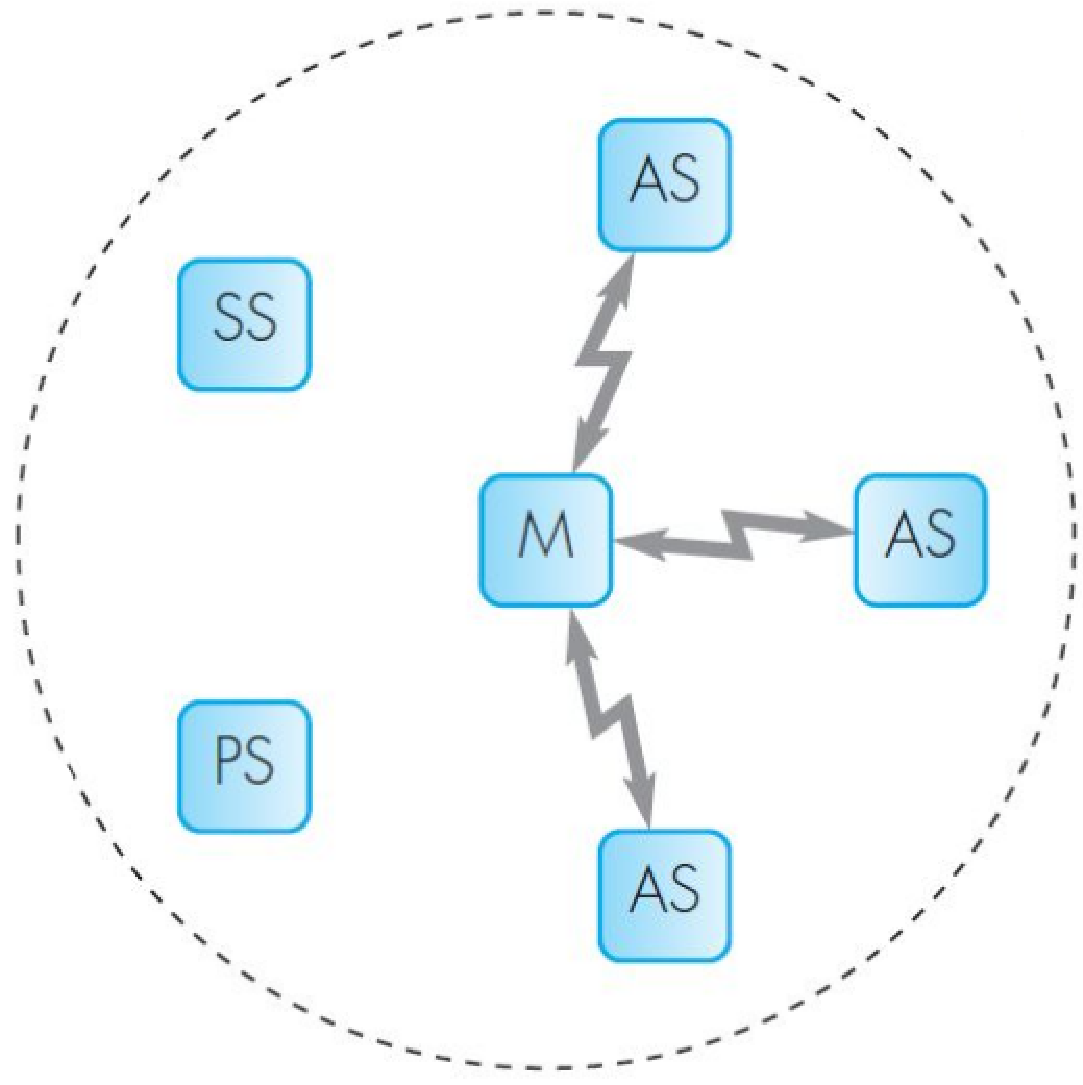
\includegraphics[width=0.4\linewidth]{img/wpan/pico1}
\end{center}

\paragraph{Scatternet:} La piconet ha al centro sempre un solo master, ma un dispositivo può appartenere a più piconet differenti, portando a una scatternet
\begin{center}
	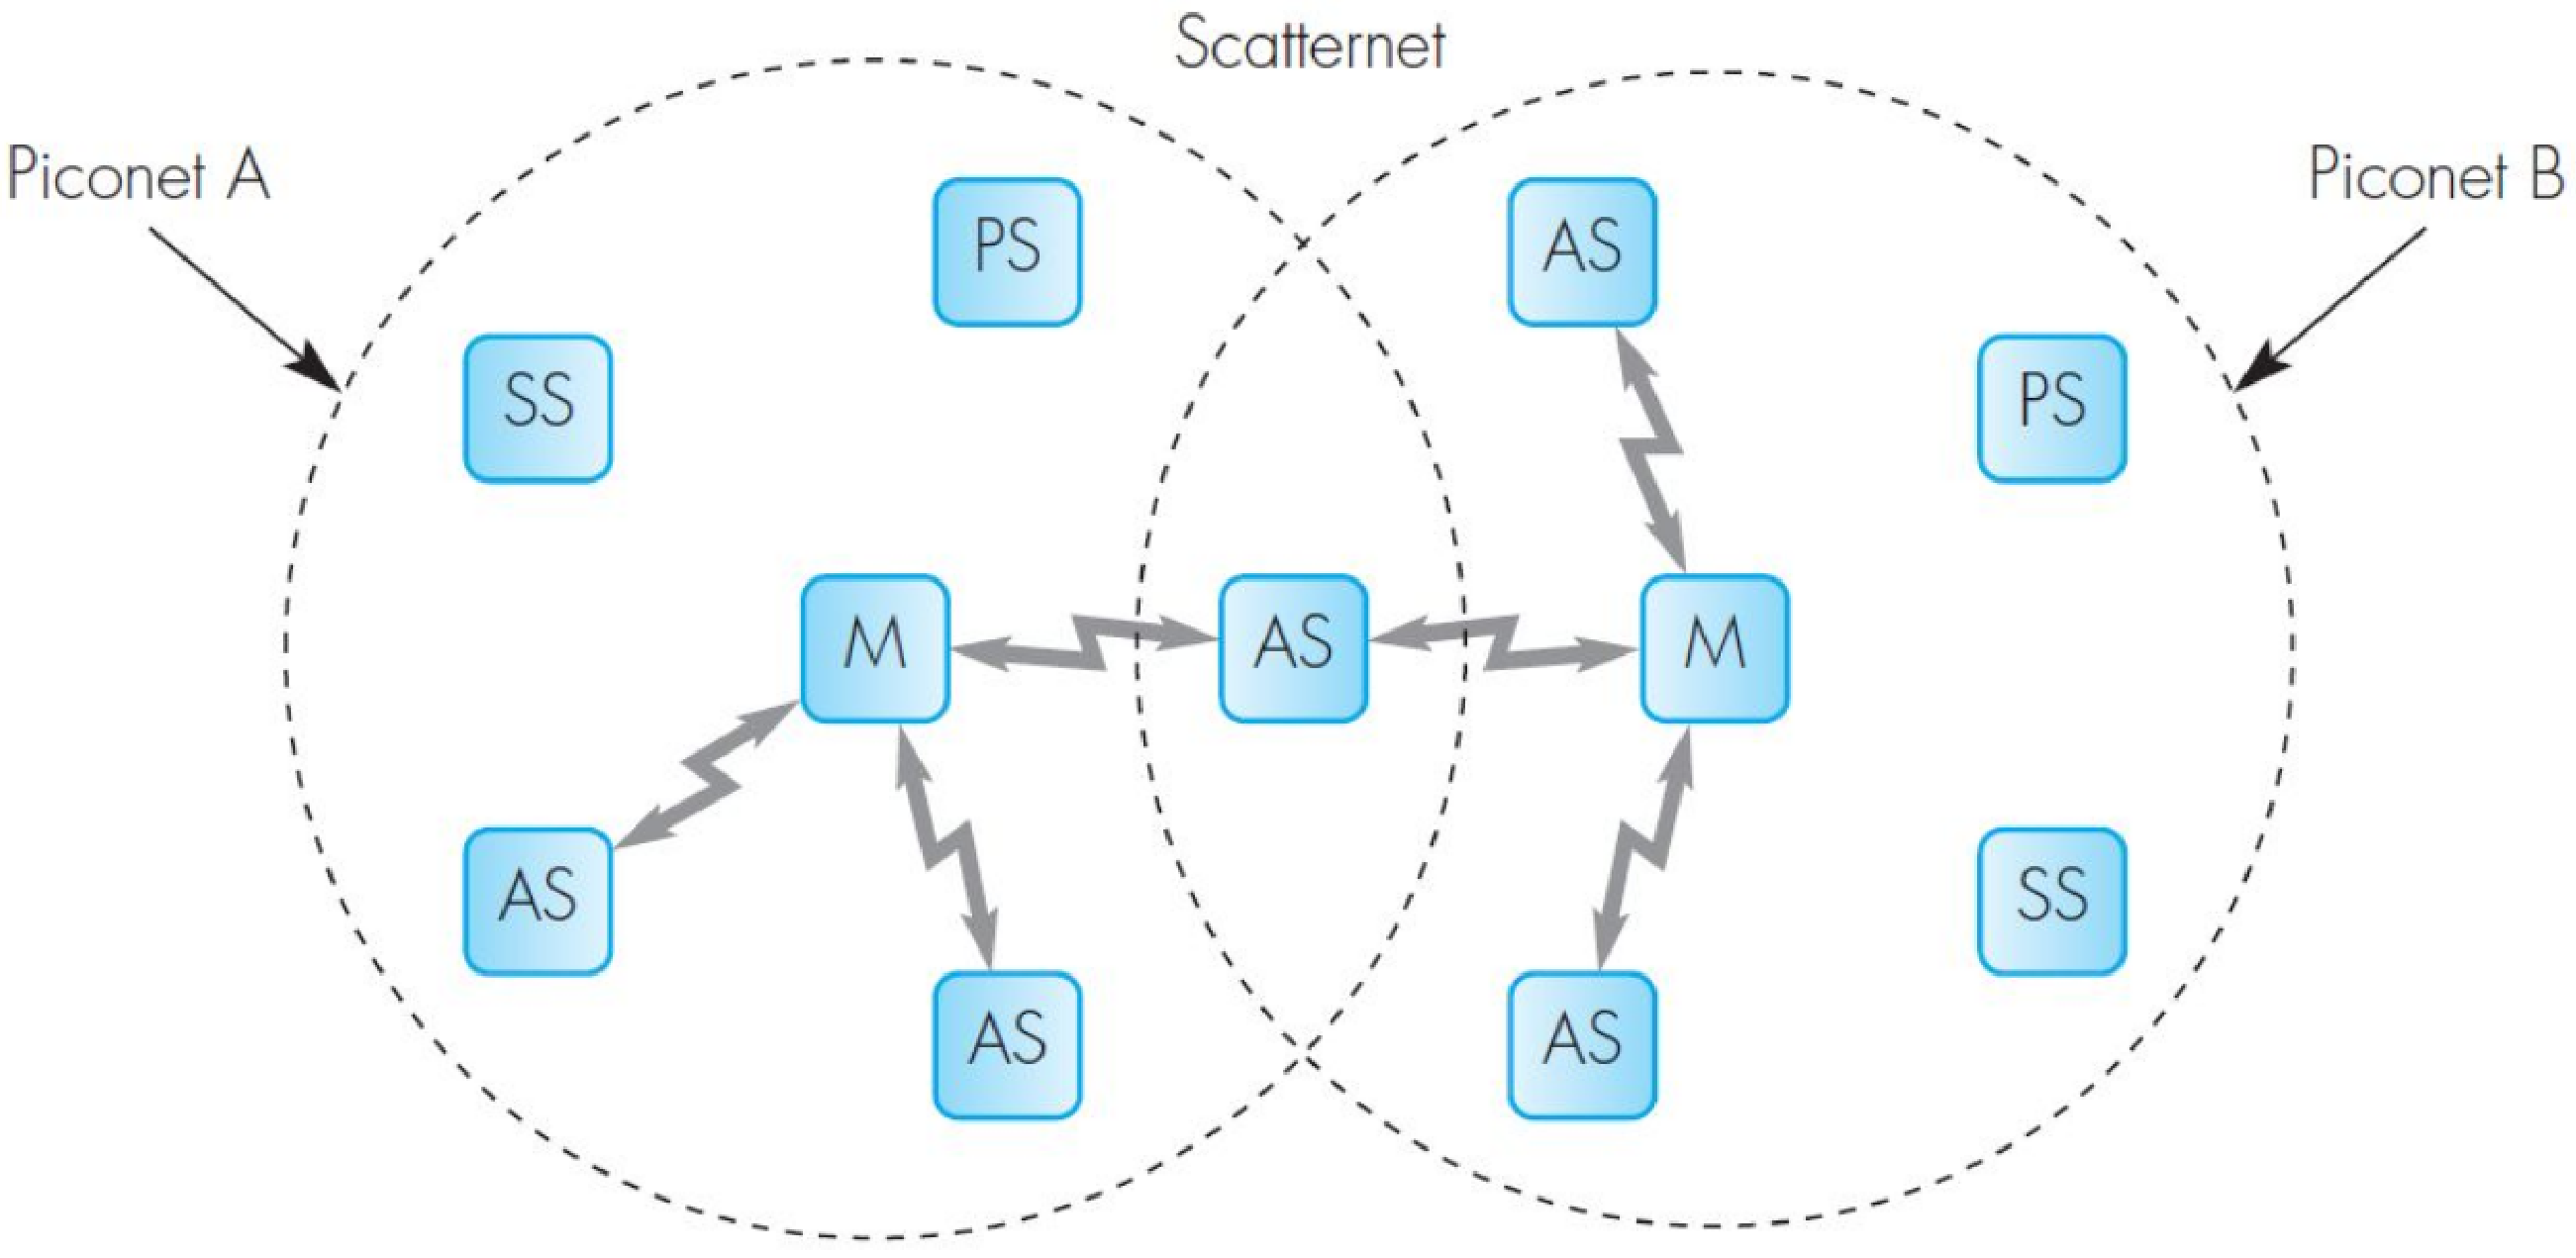
\includegraphics[width=0.8\linewidth]{img/wpan/scatter}
\end{center}

I master lavorano sempre in maniera completamente autonoma. Un AS attivo in due piconet diverse avrà indirizzamento diverso sulle due reti.

\subsubsection{Bluetooth Radio}

\paragraph{Specifiche radio Bluetooth 2.1:}

\begin{center}
	{
	\resizebox{0.98\textwidth}{!}{
	\renewcommand{\arraystretch}{1.2}
	\begin{tabular}{|l|l|l|}
		\hline
		& \textbf{Basic Rate (BR)} & \textbf{Enhanced Data Rate (EDR)} \\ 
		\hline
		\textbf{Topology} & \multicolumn{2}{c|}{Up to 7 simultaneous links in a logical star} \\ 
		\hline
		\textbf{Modulation} & GFSK & $\pi/4$-DQPSK and 8DPSK \\ 
		\hline
		\textbf{Peak data rate} & $1 Mbps$ & $2 Mbps$ and $3 Mbps$ \\ 
		\hline
		\textbf{RF bandwidth} & \multicolumn{2}{c|}{$220 kHz (-3 dB)$, $1 MHz (-20 dB)$} \\ 
		\hline
		\textbf{RF band} & \multicolumn{2}{c|}{$2.4 GHz$, ISM band} \\ 
		\hline
		\textbf{RF carriers} &  \multicolumn{2}{c|}{$23/79$}  \\ 
		\hline
		\textbf{Carrier spacing} &  \multicolumn{2}{c|}{$1MHz$}  \\ 
		\hline
		\textbf{Transmit power} &  \multicolumn{2}{c|}{$0.1W$}  \\ 
		\hline
		\textbf{Piconet access} &  \multicolumn{2}{c|}{FH-TDD-TDMA} \\ 
		\hline
		\textbf{Frequency hop rate} & \multicolumn{2}{c|}{1600 hops/s}\\ 
		\hline
		\textbf{Scatternet access} & \multicolumn{2}{c|}{FH-CDMA} \\ 
		\hline
	\end{tabular}}
	}
\end{center}

Per gestire le scatternet si usa FH-CDMA; anche in caso due scatternet comunichino sulla stessa frequenza si usa CDMA per poter distinguere i segnali.

\paragraph{Classi di potenza:} I dispositivi Bluetooth si differenziano in base alla classe di potenza
\begin{itemize}
	\item Power class 1: $100 mW$ 100 metri (senza ostacoli)

	\item Power class 2: $2.5 mW$ 10 metri (più tipico per BT)

	\item Power class 3: $1 mW$ 1-2 metri
\end{itemize}

\paragraph{Comunicazione nelle piconet:} Per comunicare ll'interno di una piconet vengono usate
\begin{itemize}
	\item \textbf{Frequency Hopping FH}: la frequenza è decisa dal master e condivisa agli slave nella piconet

	\item \textbf{Time Division Duplex TDD}: la comunicazione tra master e slave è gestita in tempo e alternata, prima comunica il master con lo slave, poi si invertono, con slot di $625\mu s$ (inclusa una guardia di $220 \mu s$)

	\item \textbf{Time Division Multiple Access TDMA}: per gestire più dispositivi nello stesso momento
\end{itemize}
\begin{center}
	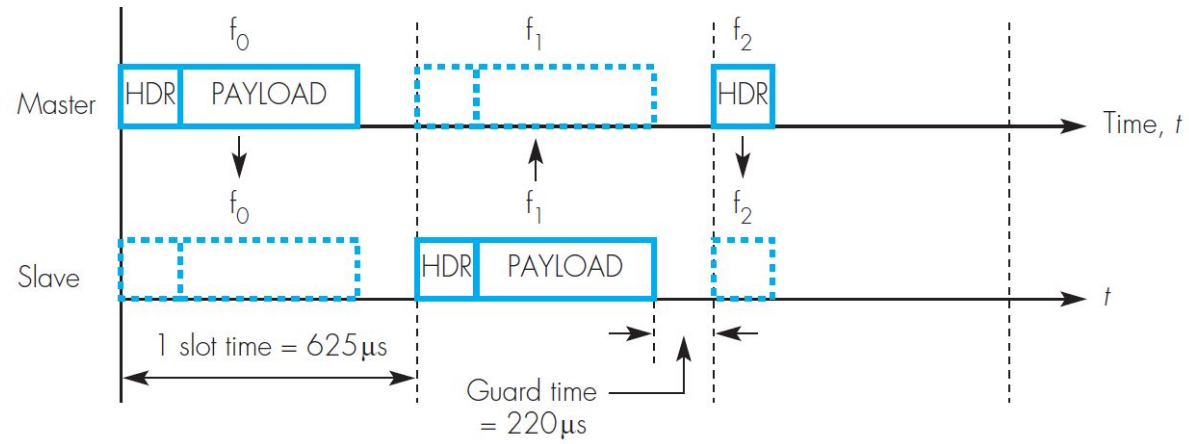
\includegraphics[width=0.9\linewidth]{img/wpan/picocomm}
\end{center}

%End L5

Esempio a più dispositivi: 
\begin{center}
	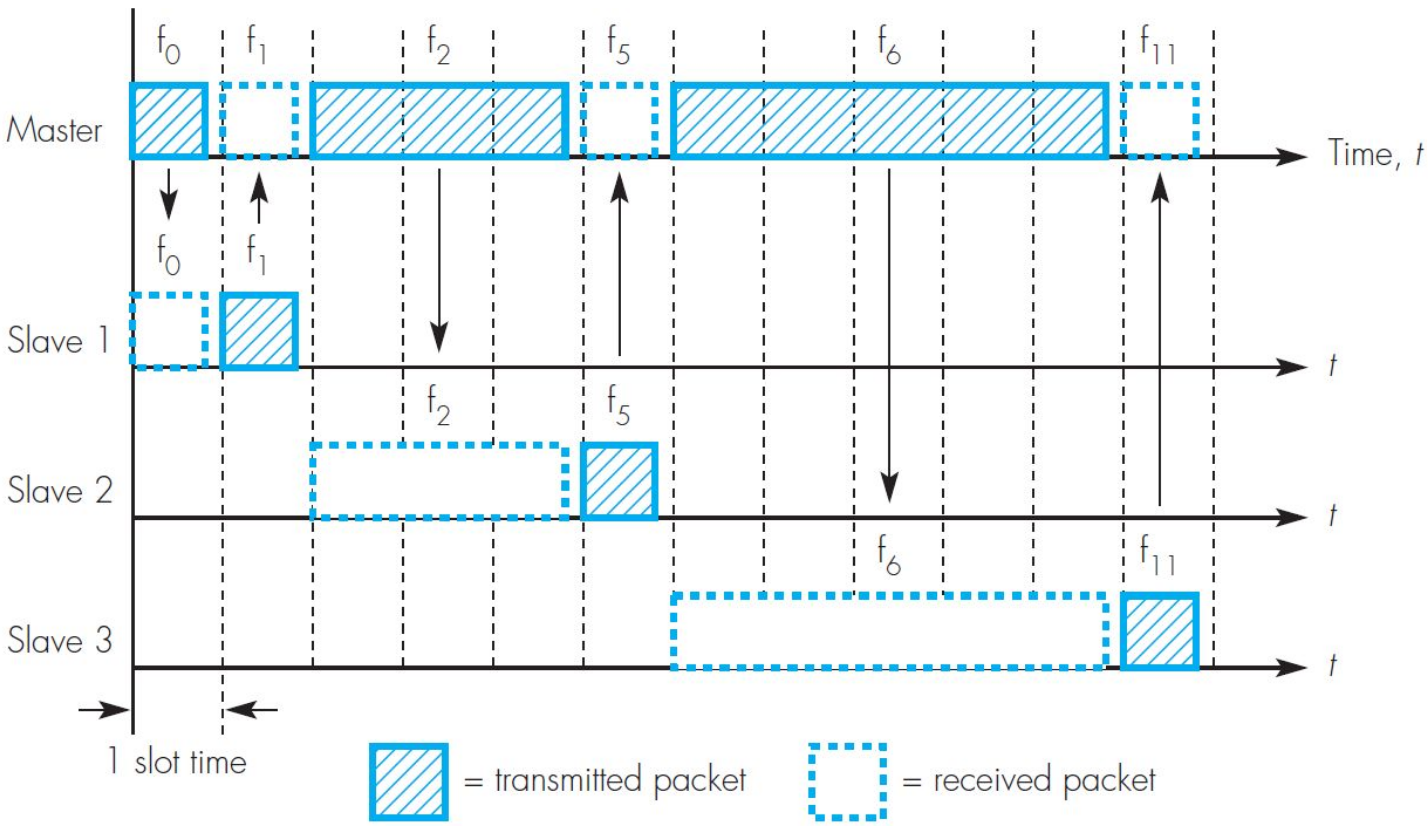
\includegraphics[width=0.9\linewidth]{img/wpan/picocomm2}
\end{center}

Nelle frequenze pari la comunicazione è da master a slave, nelle frequenze dispari viceversa. Più slave vengono coordinati tramite TDMA: il master decide chi può comunicare in quale slot di tempo. 

La \textbf{dimensione dei messaggi} può essere di 1, 3 o 5 slot di tempo consecutivi (dispari per mantenere l'alternanza in TDD). Nell'header di ogni pacchetto è indicata la dimensione.

La frequenza usata dal frequency hopping è data dal numero di timeslot passati, non dal numero di messaggi: al time slot 5 viene usata la quinta frequenza $f_5$, anche se sono stati inviati solo 3 messaggi. 

Per una singola trasmissione (messaggio) viene mantenuta la stessa frequenza (non cambia a metà). All'interno della piconet tutti i clock devono essere sincronizzati.

\paragraph{Scatternet:} Nel caso di una scatternet, ogni piconet che la compone è completamente divisa: diverse frequenze, diverso clock e di conseguenza completa autonomia. Un AS connesso a più piconet deve essere in grado di gestire le due connessioni indipendentemente (anche a livello di capacità fisica del processore).

Su 79 canali, cambiati ogni $625 \mu s$, può capitare una sovrapposizione (quindi interferenza), possibili soluzioni sono: 
\begin{itemize}
	\item FH su un numero ridotto di canali, e.g., ogni piconet su 20 canali e si spera non ci sia sovrapposizione in quei 20
	
    \item Si usa CDMA per evitare interferenze; il master comunica un codice ortogonale ai dispositivi all'interno della piconet (soluzione effettivamente usata)
\end{itemize}

%%%%%%%%%%%%%%%%%%%%%%%%%%%%%%%%%%%%%%%%%%%%
% TODO: From here
%%%%%%%%%%%%%%%%%%%%%%%%%%%%%%%%%%%%%%%%%%%%

\subsubsection{Baseband}

\paragraph{Tipologie di servizio:} Offre due possibili canali logici: 
\begin{itemize}
	\item \textbf{Synchronous Connection-Oriented Link (SCO)} point-to-point:
	\begin{itemize}
		\item canale audio/voce di $64kbps$ bidirezionale
		\item il master riserva una coppia di slot adiacenti ad intervalli regolari
		\item previsti fino al massimo di 3 canali SCO attivi contemporaneamente
		\item traffico real time
	\end{itemize}
	Garantiscono un bit rate fisso, un canale riservato, usato per casistiche sensibili al delay (real time).
	
	\item \textbf{Asynchronous Connectionless Link (ACL)} point-to-multipoint:
	\begin{itemize}
		\item canali ACL occupano gli slot rimanenti
		\item traffico dati con ciascuno degli slave
		\item un solo ACL contemporaneo fra master e uno slave
		\item traffico best effort (nessuna garanzia di delay)
	\end{itemize}
	Bit rate non costante, permette una qualità maggiore ma senza nessuna garanzia.
\end{itemize}
\begin{center}
	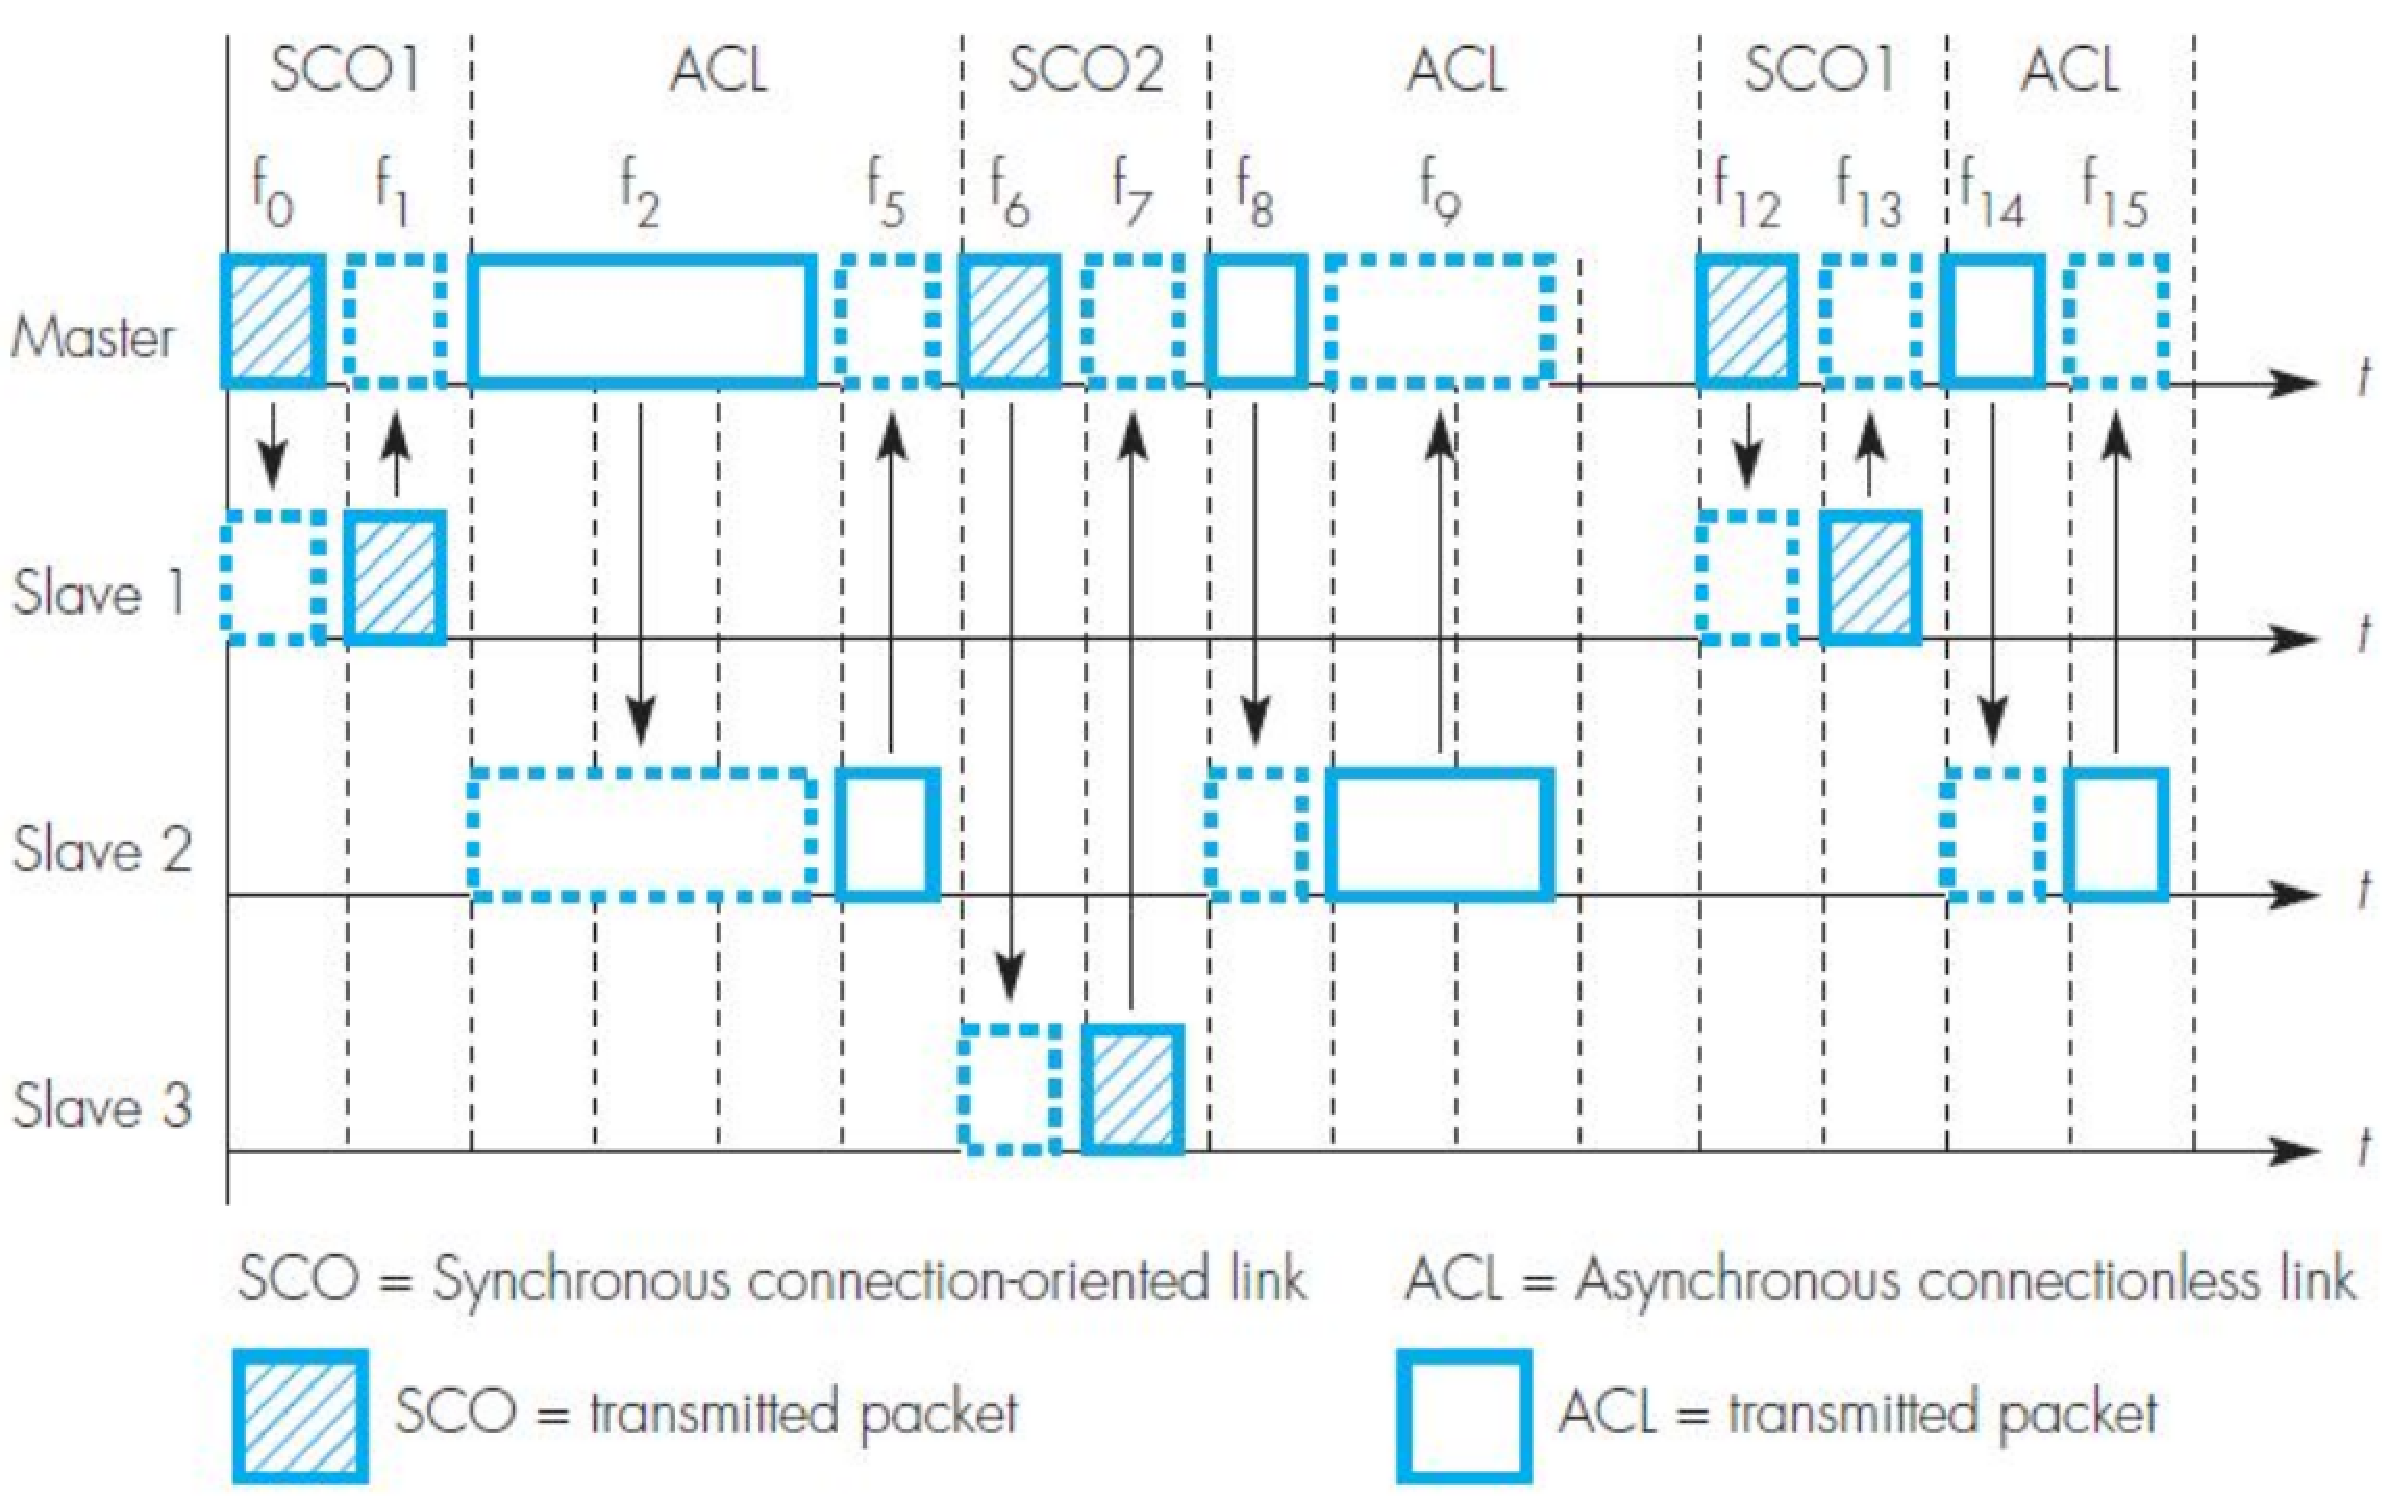
\includegraphics[width=0.9\linewidth]{img/wpan/scoacl}
\end{center}

\paragraph{Formato pacchetti:} 
\begin{center}
	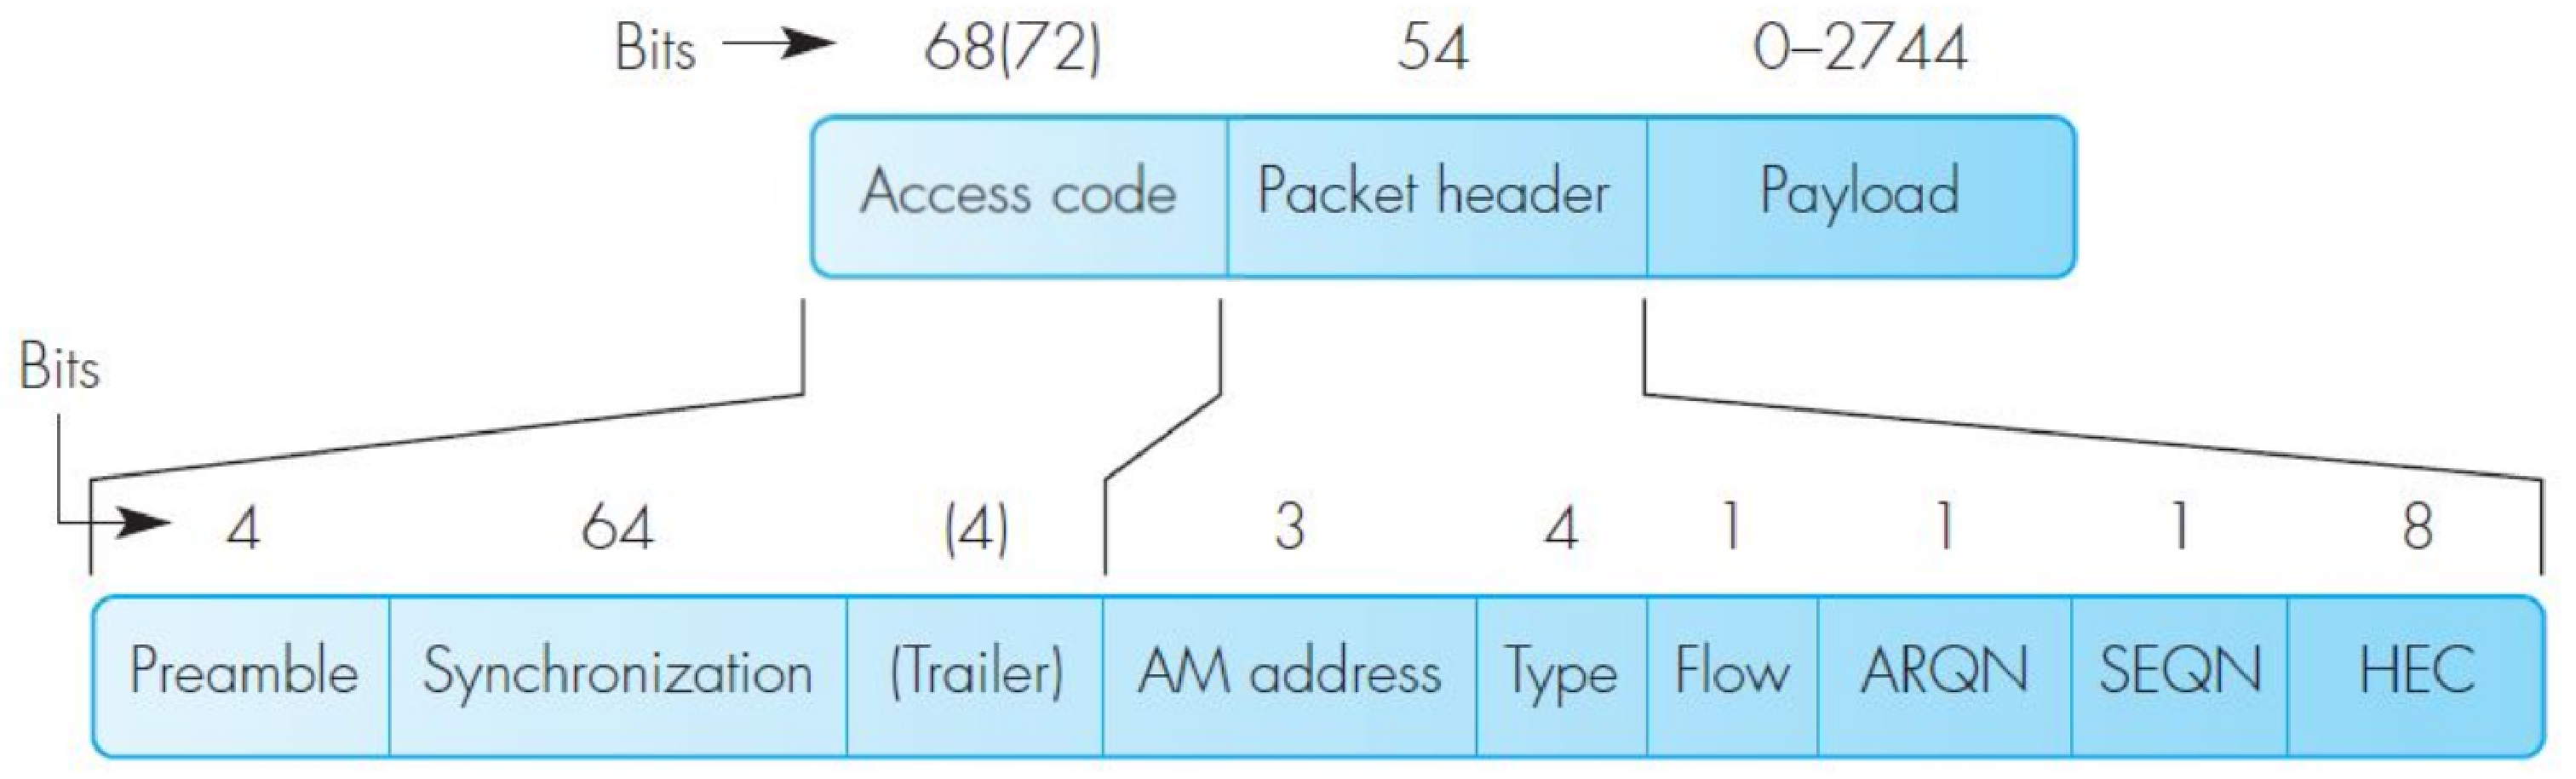
\includegraphics[width=0.9\linewidth]{img/wpan/basebandpacket}
\end{center}
Access code: utilizzato per sincronizzazione e identificazione. Può essere di 3 tipi:
\begin{itemize}
	\item Channel Access Code (CAC): identifica la piconet (derivato dai 48 bit dell'indirizzo hardware del master)
	\item Device Address Code (DAC): derivato dall'indirizzo hardware dello slave ed è usato dal master per chiamare il dispositivo (paging)
	\item Inquiry Address Code (IAC): usato per trovare l'indirizzo di un dispositivo vicino (durante la fase di inquiry)
\end{itemize}

Packet Header: ha diversi campi: 
\begin{center}
	    \begin{tabular}{|l|p{10cm}|}
		\hline
		\textbf{Campo Header} & \\ \hline
		AMA & Indirizzo del membro attivo della piconet \\ \hline
		Type & Identifica la tipologia del pacchetto e il formato del pacchetto SCO/ACL, numero di slot ecc... \\ \hline
		Flow & Per gli ACL: stop (1), resume (0) \\ \hline
		ARQN & 1 ACK, 0 NACK \\ \hline
		SEQN & Sequence number modulo 2 \\ \hline
		HEC & Controllo errori del campo header (1/3 FEC) \\ \hline
	\end{tabular}
\end{center}
ARQN e SEQN sono 2 bit necessari e sufficienti per il controllo degli errori (bastano grazie alla rigida struttura di comunicazione delineala al livello precedente).

%TODO Wtf, idk
Payload: contenuto effettivo del pacchetto può essere: 
\begin{itemize}
	\item SCO: 30 byte,  (FEC 0, 2/3, 1/3), che porta a massimo $64kbps$, dato che $(30 \cdot 8) \cdot (1600/6)$, ovvero $30 \cdot 8$ bit, 
	\item ACL: variabile da 0 a 343 byte
\end{itemize}

\paragraph{Controllo degli errori: }
\begin{center}
	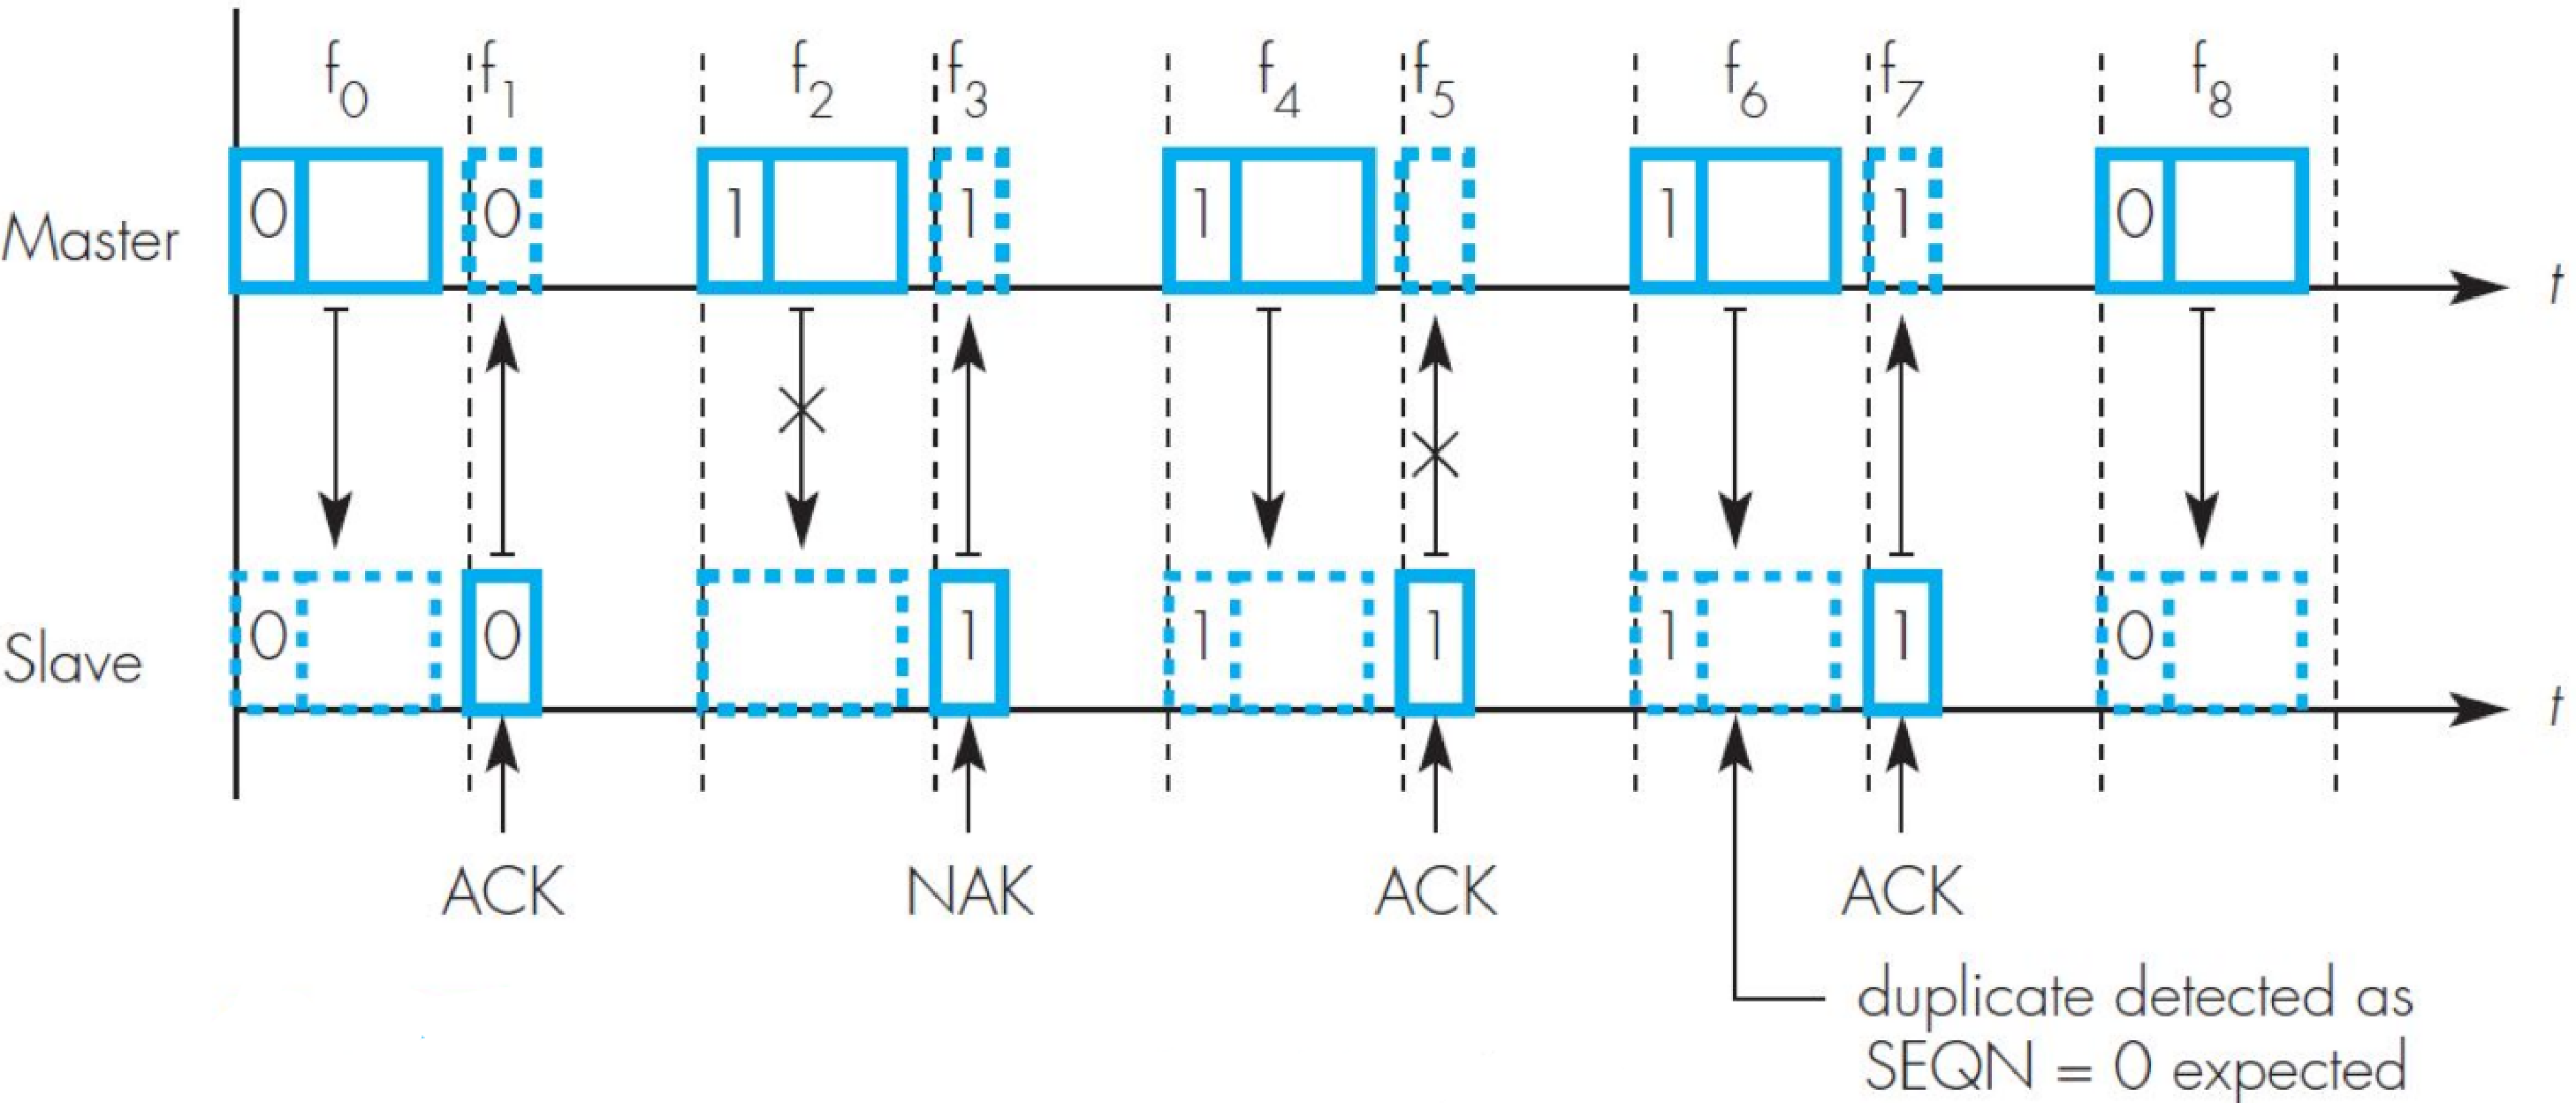
\includegraphics[width=0.9\linewidth]{img/wpan/errorcorr1}
\end{center}

All'interno del quadrato blu si vede il SEQN, mentre ACK/NACK sono indicati al di fuori.

Sequenza tipica:
\begin{itemize}
	\item Il master invia un pacchetto con un SEQN $s$
	\item lo slave risponde con un ACK ed un SEQN $s$ (lo stesso)
\end{itemize}

Possibili problemi: 
\begin{itemize}
	\item Lo slave non riceve il pacchetto: invierà un NACK per indicare la mancata ricezione, nello slot successivo deve parlare lo stesso dato che "è il suo turno", sa che ci sarà un SEQN pari a $\neg s$ ma non ha ricevuto nulla e lo indica con il NACK. "Non ho ricevuto e mi aspettavo questo"
	\item Se il master non riceve risposta dallo slave (ACK perso), il pacchetto viene re-inviato, con la possibilità di inviare un duplicato, ma meglio che perdere pacchetti
	\item Lo slave riceve un duplicato e se ne accorge in quanto il SEQN è uguale a quello precedente (il master non ha ricevuto l'ACK, non è cambiato il SEQN, quindi è una ritrasmissione del pacchetto precedente)
\end{itemize}
La rigidità dell'alternanza tra master e slave permette di rendere minimale lo spazio necessario per effettuare il controllo degli errori.

\subsubsection{Link Manager Protocol}
\paragraph{Transizioni di stato:}
\begin{center}
	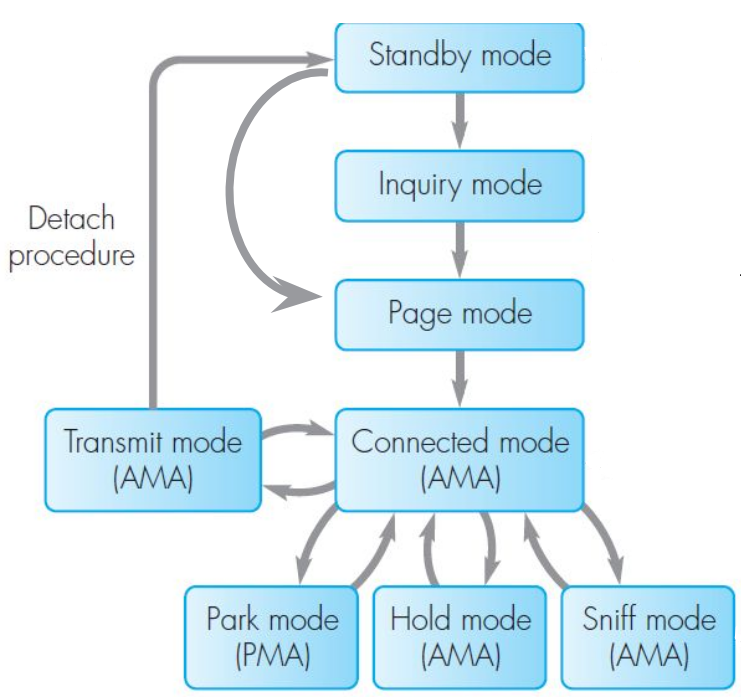
\includegraphics[width=0.55\linewidth]{img/wpan/lmpst}
\end{center}

\paragraph{Standby Mode:} A dispositivo "appena acceso" entra in standby mode, non membro di alcuna piconet, minimo consumo.

\paragraph{Inquiry mode:} Periodicamente il master invia 32 messaggi consecutivi usando 32 canali (wake-up channels, la sequenza  è standard). I messaggi contengono un \textbf{IAC packet}. Gli slave periodicamente ascoltano i 32 canali per vedere se qualcuno ha mandato un IAC packet. Tutto questo in modo non coordinato.

Ogni dispositivo ascolta per $11,25 ms$, all'inizio di ogni intervallo di $1,28$ o $2,56 s$. Una volta "beccata" una trasmissione del master si aspetta un numero random di slot di tempo (random backoff) prima di trasmettere la risposta (per evitare che più slave che hanno ascoltato quella trasmissione rispondano nello stesso momento). Possiamo farlo dato che adesso l'unica cosa che sappiamo è il clock del master, ricevere un qualsiasi segnale del master permette di sincronizzarsi con la piconet. La risposta contiene il Blouetooth Device Address dello slave e la classe, per indicare il tipo di dispositivo.

Lo slave ascolta su una delle 32 frequenze di wake-up, mentre il master invia sempre su tutte e 32. In questo modo, ascoltando per un certo periodo di tempo, se, anche solo \textit{vagamente} allineato, lo slave vedrà la comunicazione del master (insomma, prima o poi la becca). Poi c'è un random backoff di un certo numero di slot ti tempo prima di rispondere al master per richiedere il FH, DAC e AMA, inviato su 16 dei 32 canali di wake up (simile a prima).

Per finalizzare la connessione mancano le frequenze di hopping: si usano 16 delle 32 frequenze standard, per mandare: Device Access Code DAC, la sequenza di FH e l'Active Member Address AMA dello slave.

Lo slave risponde con DAC e ACK, poi può cominciare la comunicazione.
\begin{center}
	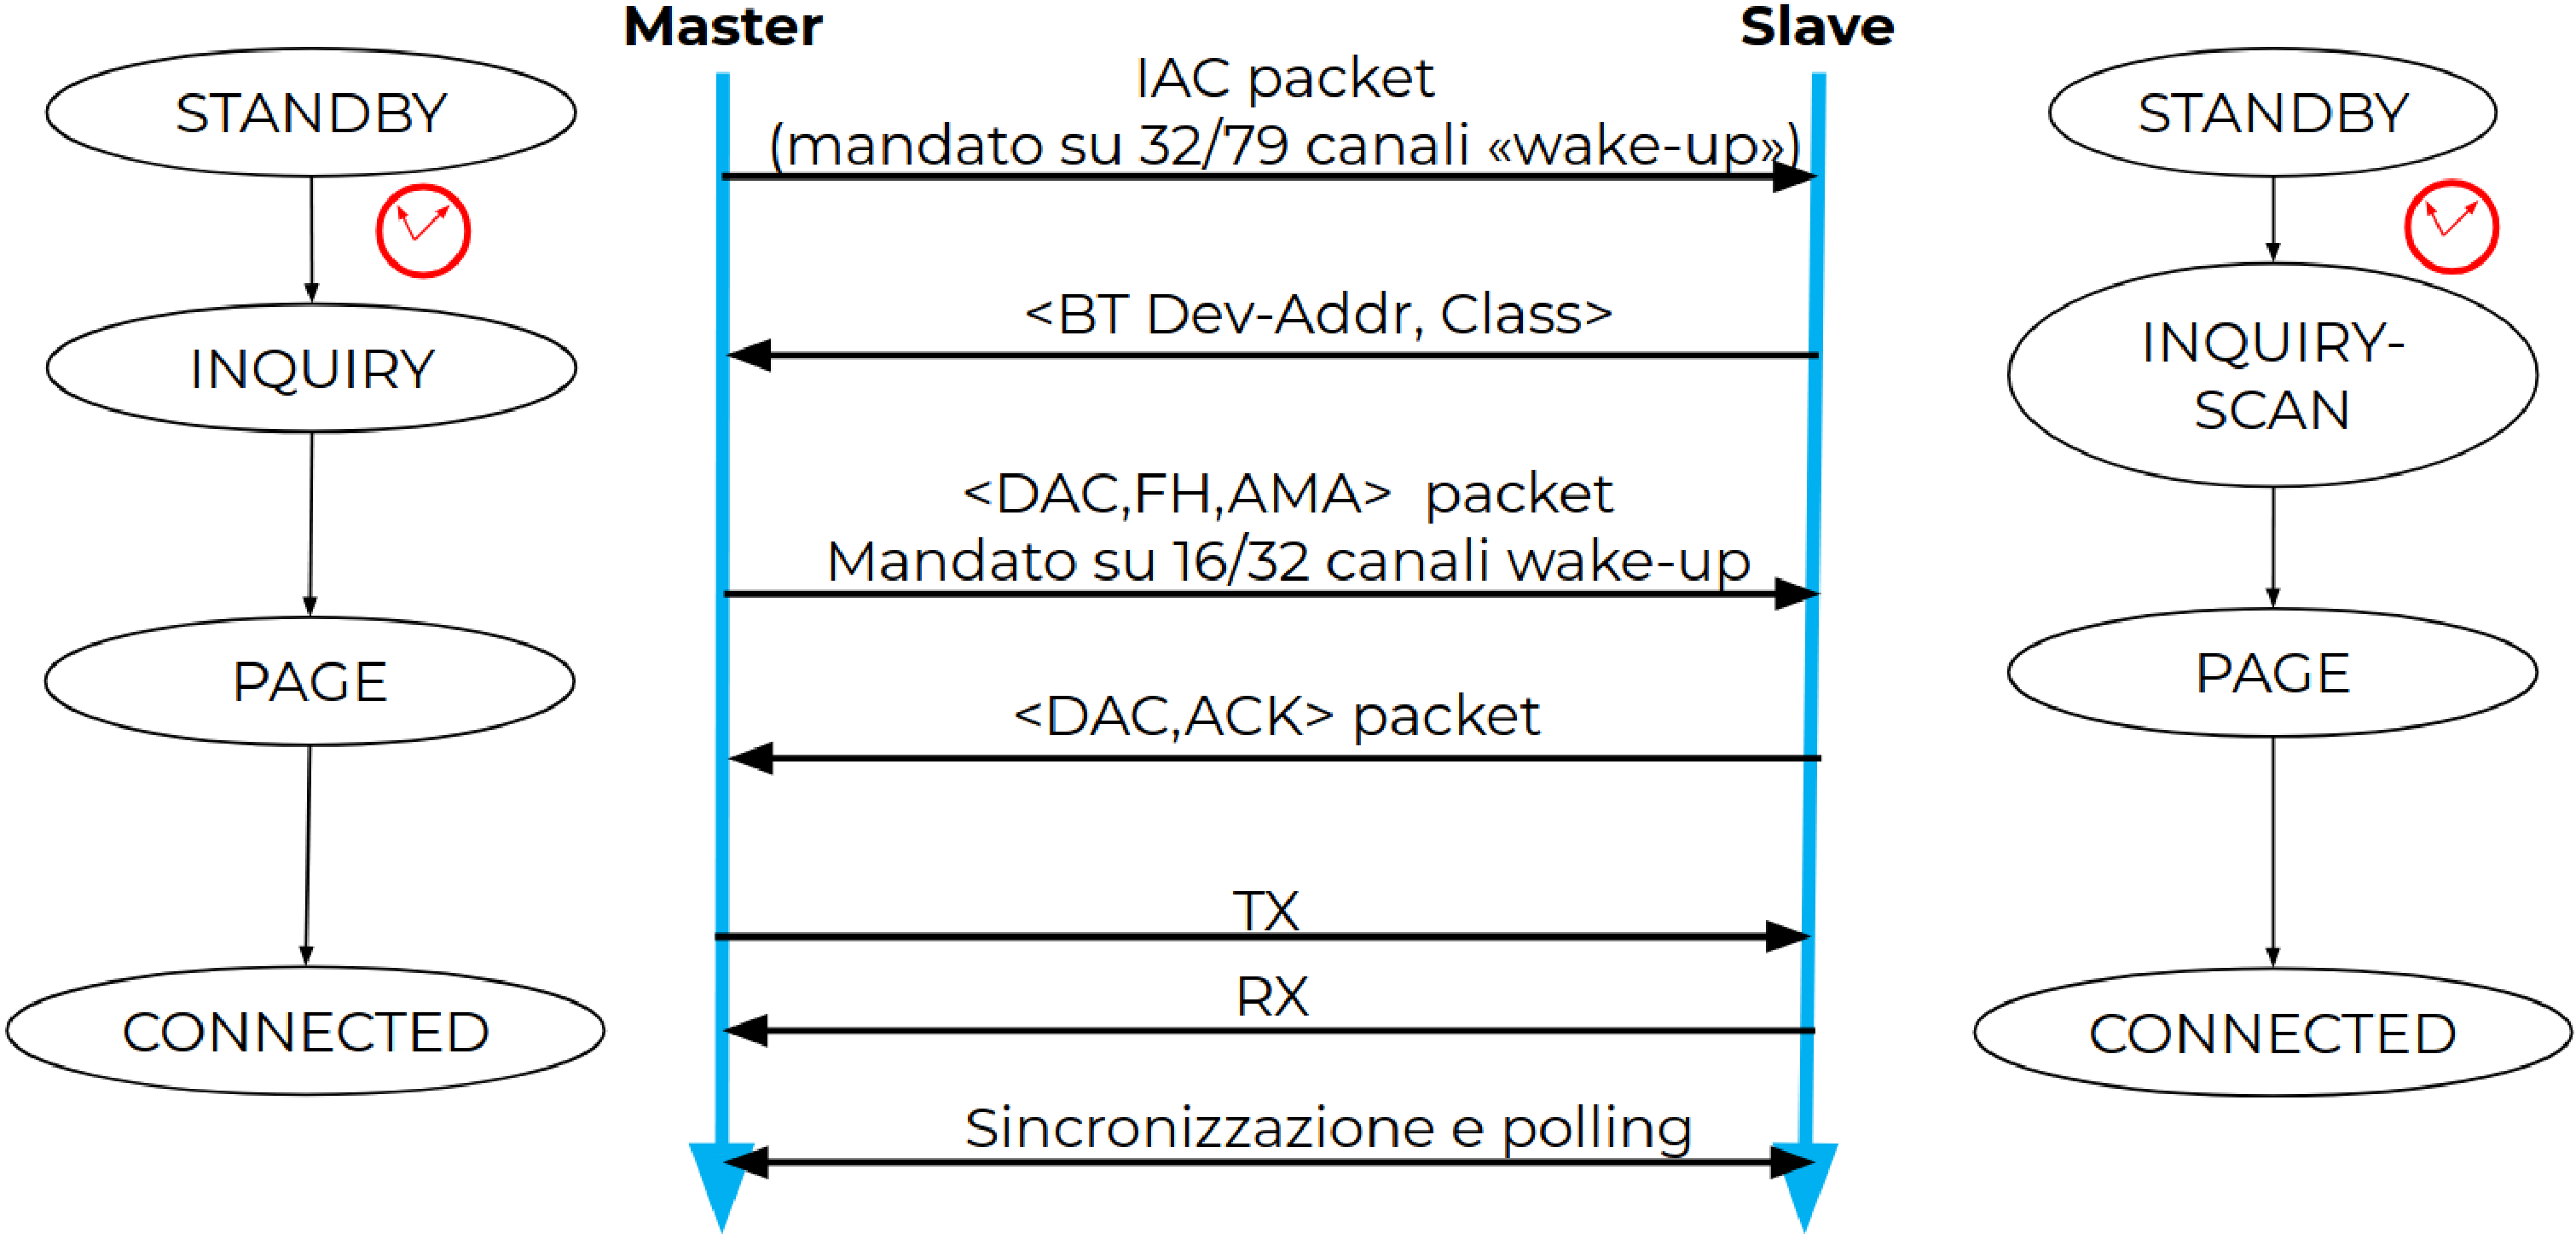
\includegraphics[width=0.95\linewidth]{img/wpan/inquiry1}
\end{center}

%End L6

\paragraph{Fase di paging:} Dopo la fase di inquiry, il master invia messaggi di paging per richiamare il dispositivo target, fornire tutti i dati di sincronizzazione necessari e stabilire definitivamente la connessione.

\paragraph{Altri stati:} Un dispositivo "attivo" può essere:
\begin{itemize}
	\item \textbf{Connected}: connessi ma non stiamo trasmettendo, sta solo ascoltando il master.
	\item \textbf{Transmit}: quando deve trasmettere va in transmit mode.
\end{itemize}
Entrambe queste modalità fanno uso del AMA. 

Entrambe queste modalità consumano batteria (transmit un po' di più, ma comunque consumano), di conseguenza ci sono 3 \textbf{stati di power saving} (in ordine discendente di consumo): 
\begin{itemize}
\item \textbf{Sniff Mode}: non ascolta tutti gli slot (mantiene AMA)
\item \textbf{Hold Mode}: ascolta solo canali SCO (mantiene AMA)
\item \textbf{Park Mode}: rimane membro della piconet ma rilascia l'AMA e gli viene assegnato un PMA. Periodicamente ascolta i messaggi che il master invia in broadcast a tutti i membri parked. Rimane sincronizzato con clock e FH del master. Può tenere spenta la radio mentre non ascolta, per risparmiare batteria (ma ogni tanto va accesa per risincronizzare il clock, bisogna mantenere quello del master)
\end{itemize}

\subsubsection{Logical Link Control and Adaptation Protocol L2CAP}
Sempre presente in tutti i dispositivi Bluetooth, ma è il primo livello software (richiede combinazione di pacchetti a livello fisico). Non viene usato per l'audio (maggior parte dei canali SCO).

Supporta solo canali ACL. Offre 3 tipi di \textbf{canali logici}:
\begin{itemize}
	\item \textbf{Connectionless}: unidirezionale, ad esempio tra broadcast e slave, per quando non c'è la necessità di instaurare una connessione
	\item \textbf{Connection-oriented}: bidirezionale e supporto QoS (richiedere una certa qualità del canale)
	\item \textbf{Signaling}: bidirezionale usato per messaggi di controllo master/slave, controllo di un livello superiore
\end{itemize}

\paragraph{Formato dei pacchetti:}
\begin{center}
	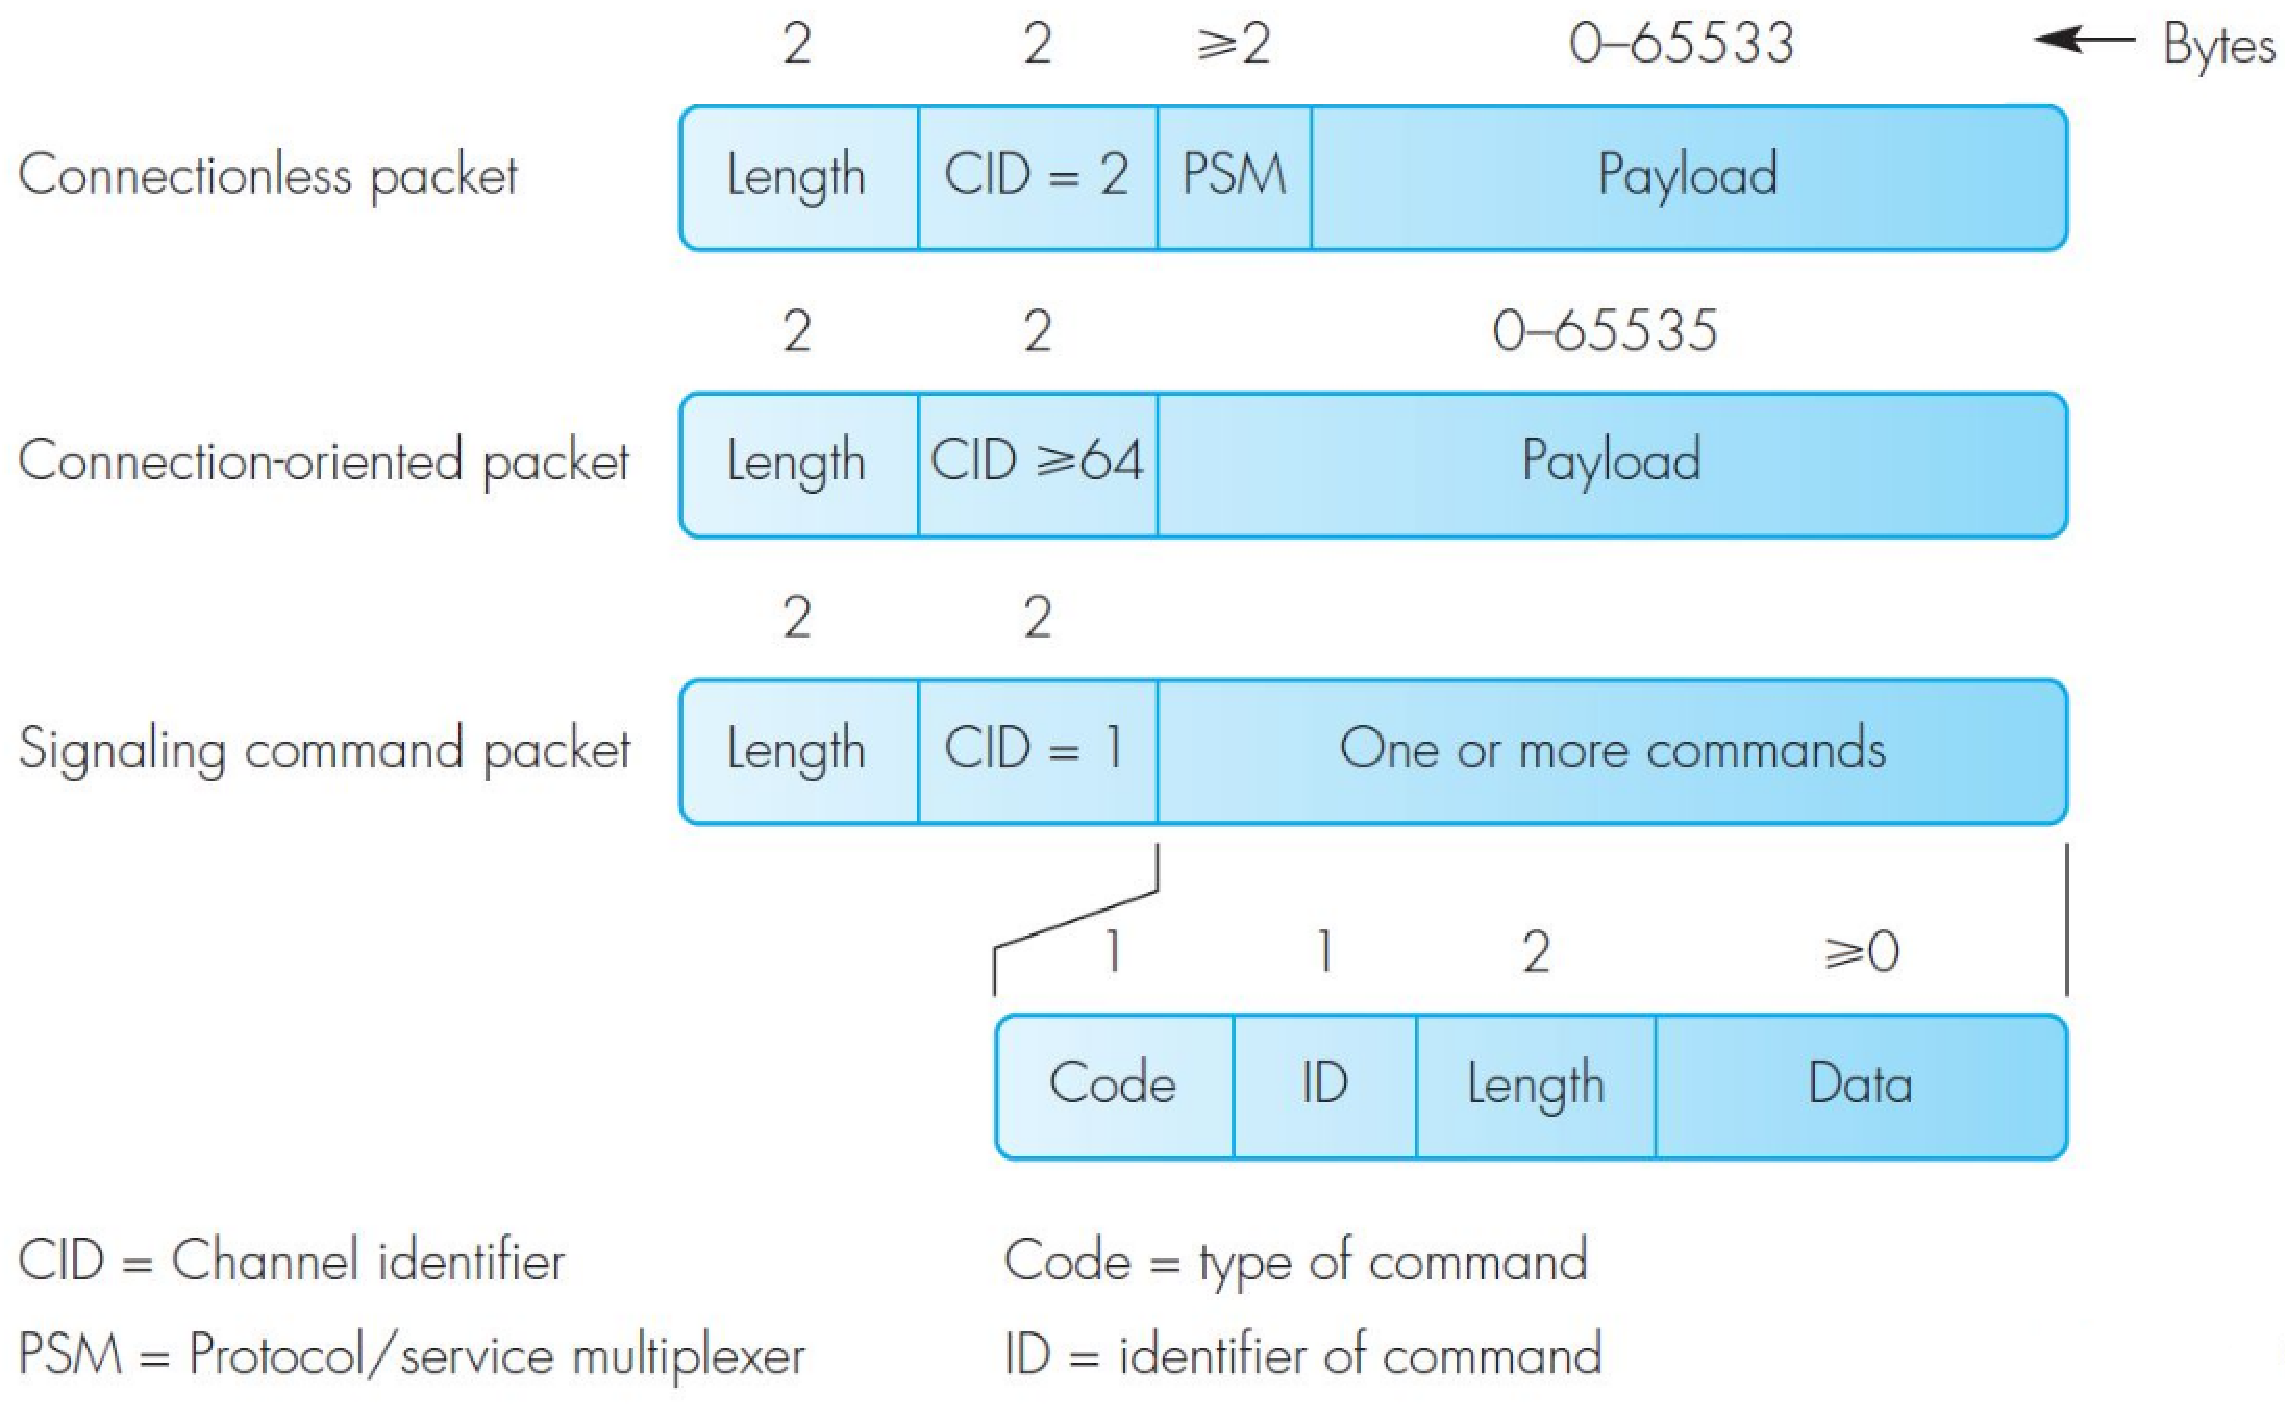
\includegraphics[width=0.9\linewidth]{img/wpan/l2cappacket}
\end{center}
La dimensione è segnata in byte, i pacchetti sono molto più grandi di quelli a livello baseband, la \textbf{segmentazione ed assemblamento} dei frame inviati a livello baseband viene \textbf{effettuata da L2CAP} (stile ethernet e trasporto, il messaggio sopra viene ricostruito, anche se sotto è diviso in più messaggi).

I valori del Channel Identifier possibili sono: 
\begin{itemize}
	\item CID $= 2$: non c'è nessuna connessione, pacchetto per connectionless
	\item ID $\geq 64$: pacchetto connection-oriented, il numero indica la connessione
	\item CID $=1$: usato per i pacchetti di signaling/controllo
\end{itemize}

Al posto di avere dati relativi all'applicazione, il payload di un pacchetto di controllo contiene
\begin{itemize}
	\item Code: codice per il tipo di comando 
	\item Id: per l'identificatore del comando
\end{itemize}
Poi lunghezza e dati.

\subsubsection{Service Discovery Protocol SDP}

Protocollo \textbf{client-server} in cui un server contiene le informazioni ed il client ha due possibili azioni:
\begin{itemize}
	\item ricerca di un servizio
	\item browse dei servizi (lista dei servizi disponibili su un dispositivo)
\end{itemize}
Generalmente, master chiede (client), slave rispondono alle richieste (server).

\subsection{Bluetooth Low Energy BLE}

Ha come \textbf{obiettivi}:
\begin{itemize}
	\item ridurre il consumo energetico dei dispositivi
	\item entrare nel mondo degli smart sensor (di solito difficilmente ricaricabili, quindi da fare il meno possibile)
	\item semplificare il sistema di comunicazione (l'inquiry è complicato)
	\item compatibile con più dispositivi Bluetooth
\end{itemize} 

Introduce \textbf{nuove funzionalità}: prima l'unica struttura possibile era master-slave, ma non bastava più per gli usi possibili del Bluetooth. Si aggiungono \textbf{altre strutture} di comunicazione:
\begin{itemize}
	\item \textbf{Broadcast}: più flessibile, chi è in range ascolta un broadcaster
	\item \textbf{Mesh}: struttura meno rigida, ogni dispositivo connesso a molteplici altri
\end{itemize}

Poi si aggiungono funzionalità di \textbf{positioning}: 
\begin{itemize}
	\item rilevare la \textbf{presenza} di un dispositivo
	\item rilevare la \textbf{distanza}
	\item rilevare la \textbf{direzione} dal dispositivo
\end{itemize}

Si tiene la stessa banda ISM, ma i canali sono 40 al posto che 79, rendendoli più resistenti ad interferenza (anche se abbassando il data rate). 

\subsubsection{Architettura}
\begin{center}
	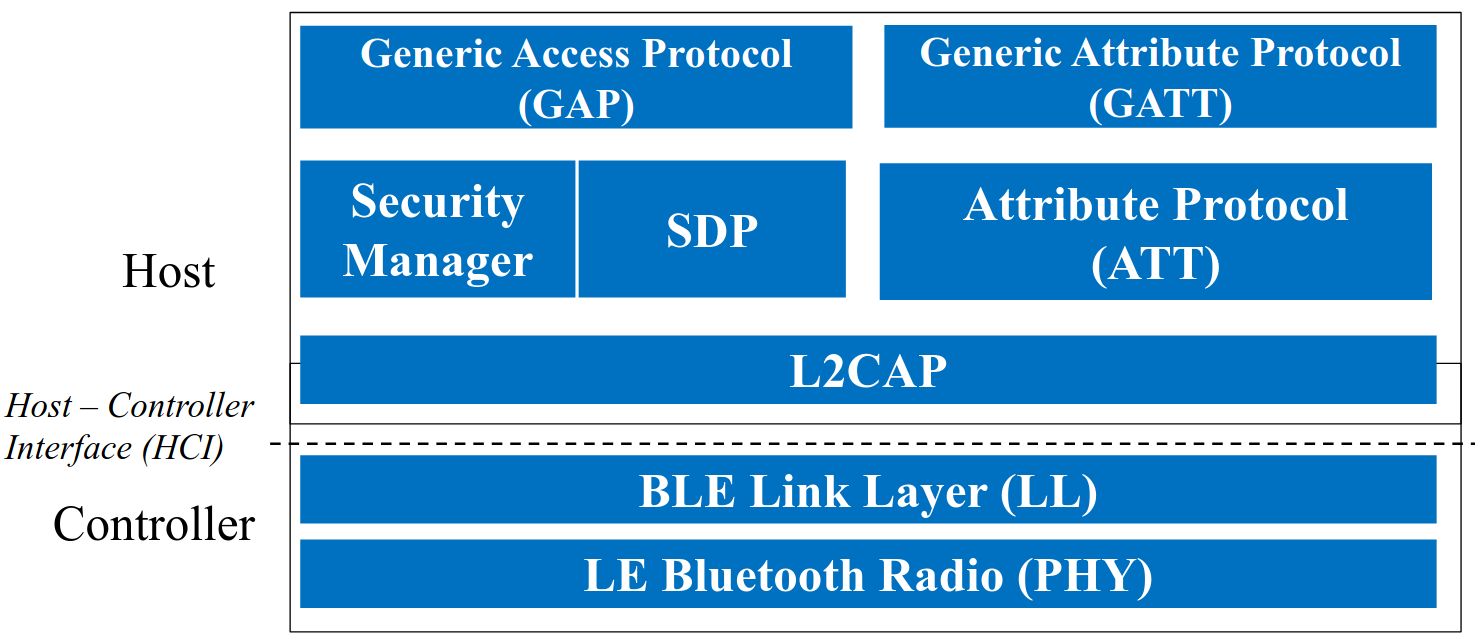
\includegraphics[width=0.8\linewidth]{img/wpan/blearch}
\end{center}

I livelli fisici cambiano in quanto è cambiata la trasmissione radio. Eccetto i primi 2, il resto è "equivalente" all'architettura del 2.1, con qualche modifica ovviamente.
%Spiega i protocolli?

\subsubsection{Classi di potenza}
\begin{center}
	\begin{tabular}{|c|c|c|}
		\hline
		\textbf{Power Class} & \textbf{Max Output Power ($P_{\text{max}}$)} & \textbf{Min Output Power$^1$} \\
		\hline
		1   & 100 mW (+20 dBm)  & 10 mW (+10 dBm)  \\
		1.5 & 10 mW (+10 dBm)   & 0.01 mW (-20 dBm) \\
		2   & 2.5 mW (+4 dBm)   & 0.01 mW (-20 dBm) \\
		3   & 1 mW (0 dBm)      & 0.01 mW (-20 dBm) \\
		\hline
	\end{tabular}
\end{center}
La perdita di potenza (il minimo è minore) sono parzialmente "controbilanciate" dallo spettro più ampio che permette una migliore ricezione.

\subsubsection{BLE Radio (PHY)}

Non cambia lo spettro, sempre $2.4GHz$ ISM, ma viene diviso in 40 canali, dei quali 37 usati per data packets, mentre gli ultimi sono usati come \textit{advertising}.

La sequenza di FH è determinata dalla formula
\begin{center}
	\texttt{channel = (curr\_channel + hop) mod 37}
\end{center}
il valore di "hop" è il "segreto" su cui fare viene fatto hopping.  

Con la Gaussian Frequency Shift Keying (GFSK) con rate di modulazione si raggiunge $1Mbps$.

\subsubsection{BLE State Machine}
\begin{center}
	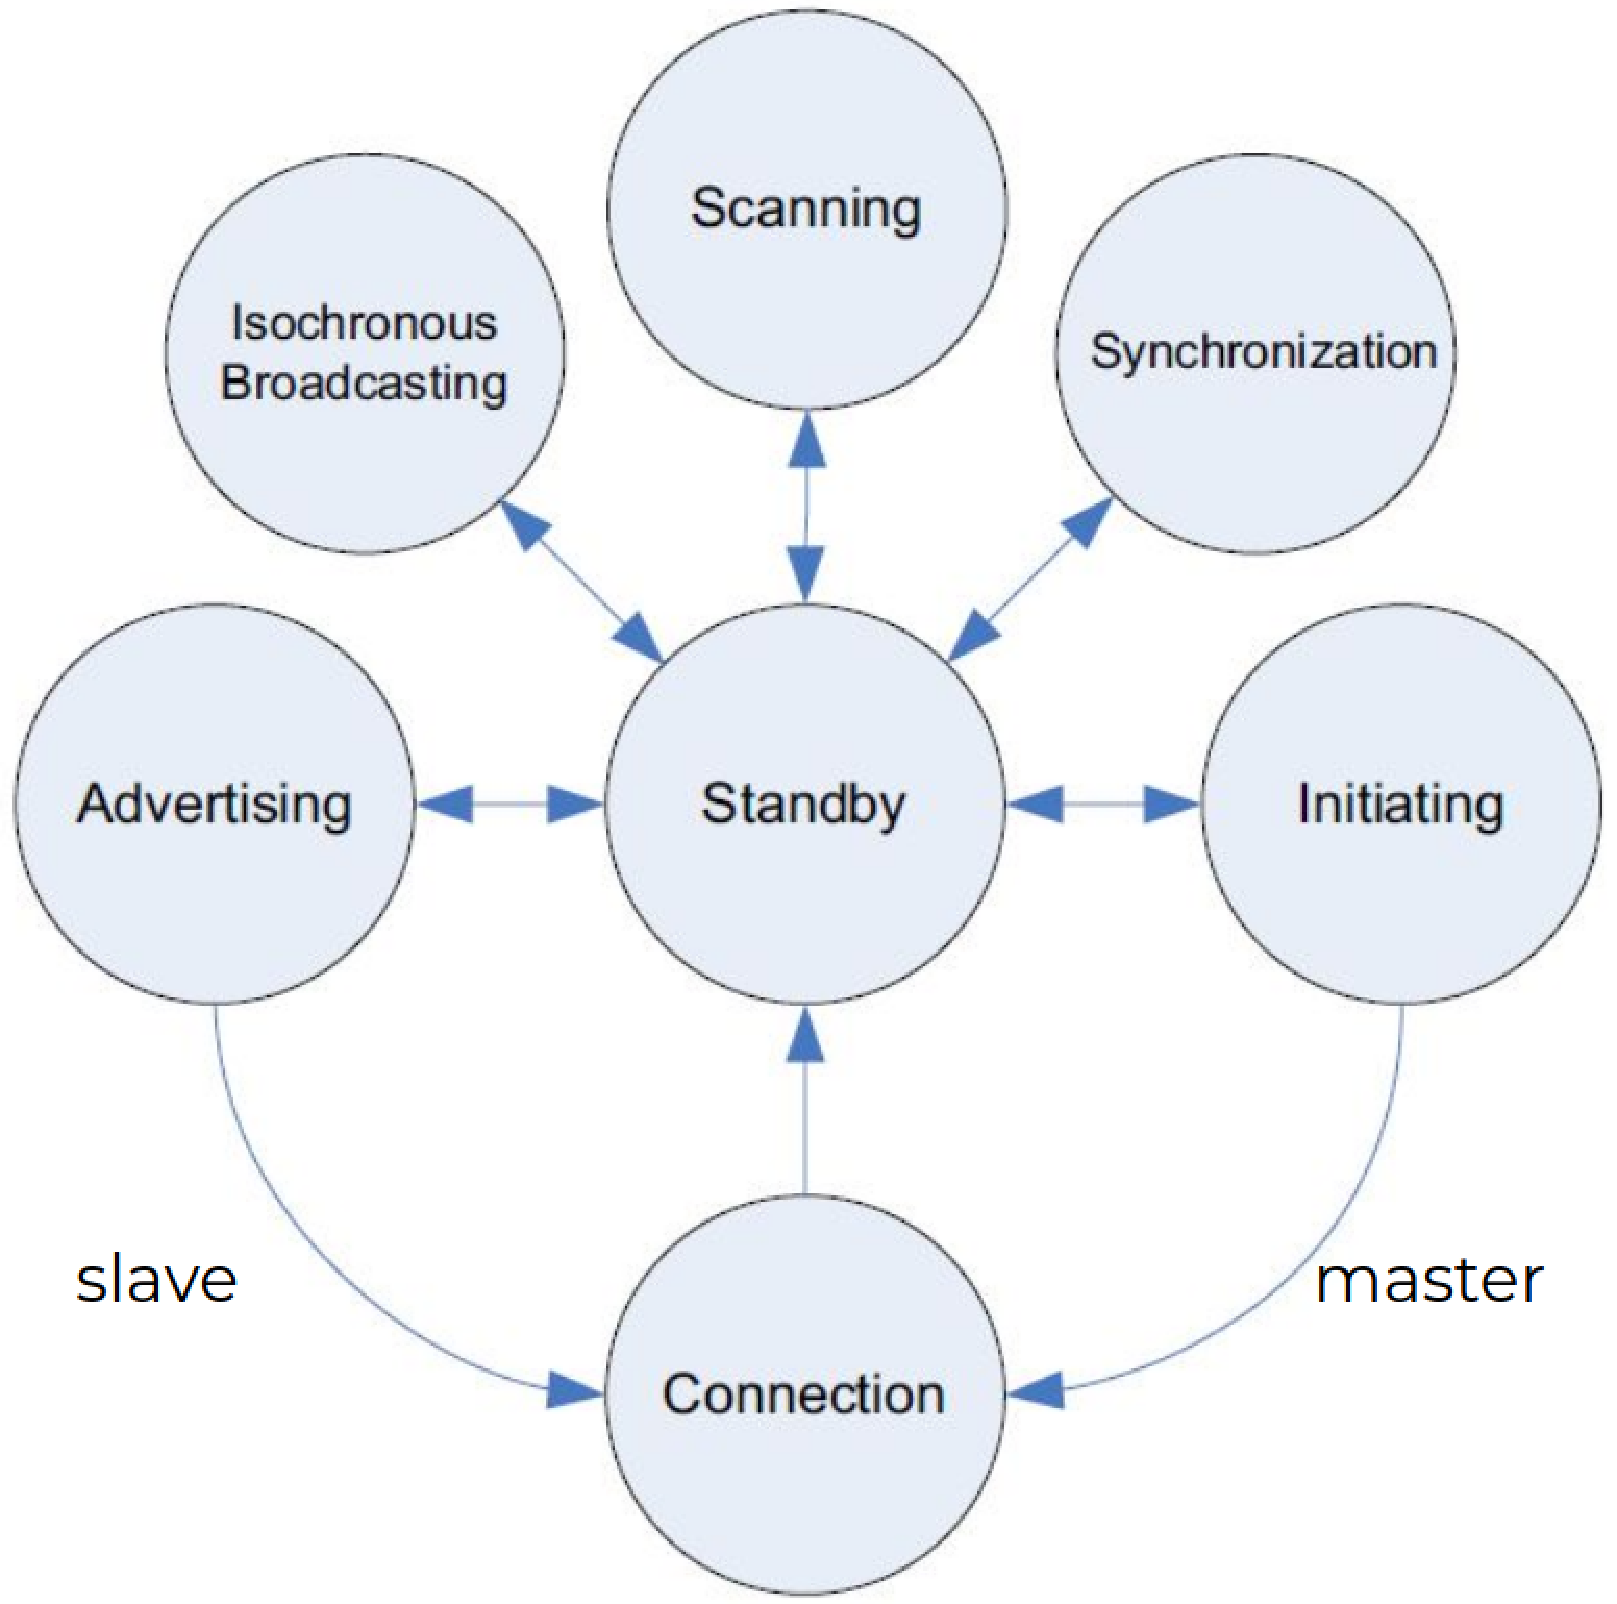
\includegraphics[width=0.6\linewidth]{img/wpan/blestate}
\end{center}
Tutti partono dallo standby.

\paragraph{Advertising:} usa i canali di advertising per farsi conoscere, non è più il master che cerca per creare la piconet, ma è lo slave che si annuncia. 

\paragraph{Initiating:} Lo stato in cui vengono ascoltati i messaggi di advertising.

\paragraph{Isochronous Broadcasting:} broadcasting periodico (isocrono) per emettere delle informazioni.

\paragraph{Scanning:} Il dispositivo si mette in ascolto.

\subsubsection{Advertising}
\begin{center}
	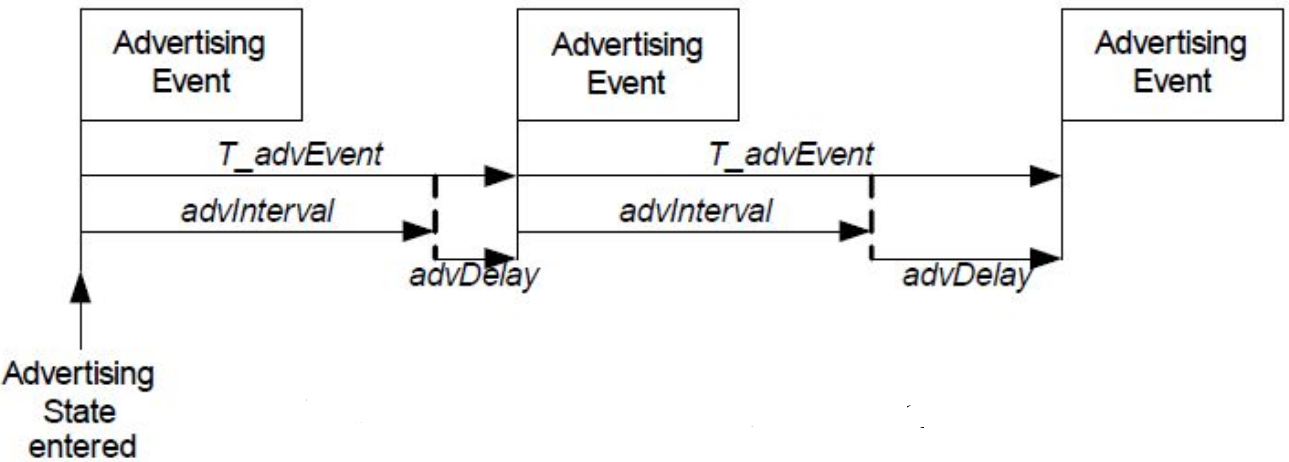
\includegraphics[width=0.85\linewidth]{img/wpan/bleadvert}
\end{center}

Ogni certa quantità di tempo viene inviato un \textbf{advertising event}, su uno o più dei canali di advertising. Il tempo tra un advertising event e l'altro è determinato da:
\begin{center}
	\texttt{T\_advEvent = advInterval + advDelay}
\end{center}
Dove
\begin{itemize}
	\item \texttt{advInterval} è un intero multiplo di $625 \mu s$ nel range $20 ms$ - $10,24s$ ed è determinato in base all'uso del dispositivo (per esempio, un sensore della temperatura non ha bisogno di inviare dati spesso quanto un accelerometro); il rate di invio determina il consumo della batteria
	\item \texttt{advDelay} è un valore psudo-random nel range $0$-$20ms$ (per evitare sovrapposizioni, sempre multiplo di $625 \mu s$)
\end{itemize}

\subsubsection{Generic Attribute Profile GATT}
Viene gestito dal modulo GATT all'interno dell'architettura, permette uno scambio di dati strutturato tra server, che offrono servizi tramite profili (e.g., fascia che misura la frequenza cardiaca avrà un Heart rate profile) e client che richiedono (e.g., smartphone che chiede la frequenza cardiaca). Ogni profilo ha i suoi dati e caratteristiche associate. Il ruolo di server o client non è fisso, può cambiare dinamicamente in base alla necessità.

\subsubsection{General Access Protocol GAP}
Un'applicazione, in base al suo scopo, può decidere uno dei "ruoli fondamentali" definiti dal GAP:
\begin{itemize}
	\item \textbf{Broadcaster}: spedisce pacchetti di advertising. Trasmissione di dati connectionless come eventi di advertising
	\item \textbf{Observer}: riceve advertising packet. Ricezione di pacchetti connectionless
	\item \textbf{Peripheral}: un peripheral device opera in slave (advertiser) mode a livello di Link Layer
	\item \textbf{Central}: un device opera in master (initiator) mode a livello di Link Layer
\end{itemize}

\paragraph{Creazione di una Connessione Unicast (peer to peer):} Host A sarà il master, B lo slave.
\begin{center}
	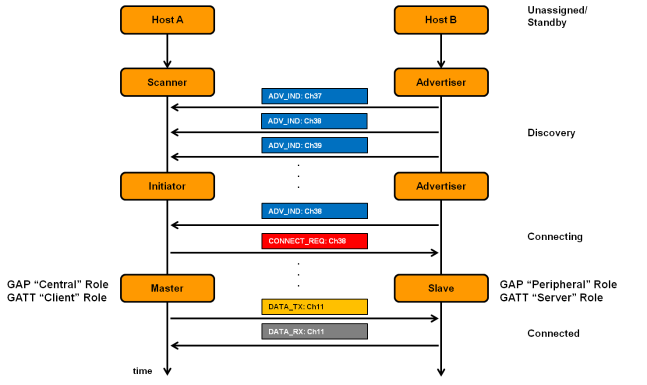
\includegraphics[width=0.98\linewidth]{img/wpan/bleunicast}
\end{center}
In questo caso è il \textbf{master che ascolta} ed il dispositivo slave è un advertiser, vuole essere trovato dal master mandando advertising packets undirected (diretti a "nessuno"), vogliono solo dire ad un initiator che c'è \textit{qualcuno} che vuole collegarsi. Vengono inviati sui 3 canali di advertising, di conseguenza il master ascolterà sugli stessi canali.

Una volta che il master "sente" il messaggio, invierà una connection request nello slot di tempo successivo (si mantiene sempre il TDD, sappiamo che nello slot di tempo successivo all'invio il dispositivo starà aspettando). Nella connection request ci sono anche le informazioni per il FH. Dopo la richiesta di connessione si passa a master e slave per la trasmissione.

\paragraph{Connessione Broadcast:} Si può anche avere una connessione "broadcast", non peer to peer, in cui abbiamo un broadcaster, che non ha interesse ad avere un master, vuole solo inviare dati.
\begin{center}
	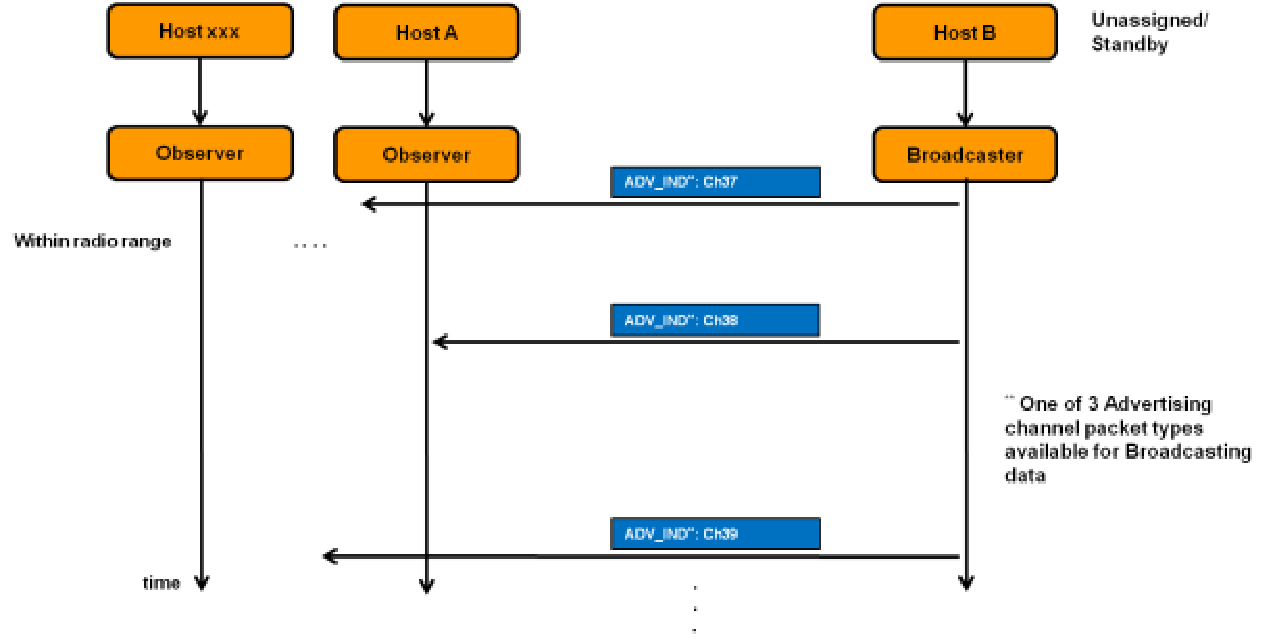
\includegraphics[width=0.98\linewidth]{img/wpan/blebroadcast}
\end{center}
Gli observer (quelli che ascoltano) saranno tutti i dispositivi all'interno del range di comunicazione.

%imgs s61, 62?
\paragraph{Passive scanning:} Lo scanner ascolta passivamente e periodicamente sui canali di advertising (solo passivo). 

\paragraph{Active scanning:} Sempre e solo usando i canali di advertising, lo scanner ascolta sul canale per poi richiedere dei dati tramite scan request (e di conseguenza otterrà la response). Quest'ultima parte è unicast con il dispositivo di broadcast.

%Fine slide 2

%End L7

%Slide 3
\subsection{ZigBee}
Sempre sotto 802.15, gli standard sono IEEE quindi siamo a livello fisico e data link.

I requisiti richiesti a ZigBee sono: 
\begin{itemize}
	\item Affidabilità
	\item Basso costo
	\item Lunga durata della batteria (molto più che Bluetooth)
	\item Bassa complessità
	\item Utilizzo delle bande ISM ($2.4GHz$ Worldwide \& $915 MHz$/ $868MHz$ in base alla zona)
	\item Scalabilità (possibile un alto numero di nodi), con diversi possibili strutture
	\item Interoperabilità tra vendors
	\item Sicurezza
\end{itemize}

Gli utilizzi sono principalmente in ambiti di domotica, IoT, monitoring, ma possono essere i può svariati, qualunque ambito richieda comunicazione di "pochi" dati tra più dispositivi con un basso consumo di energia.

Topologie di rete
Sono possibili più tipologie di rete: stella, albero, mesh.
\begin{center}
	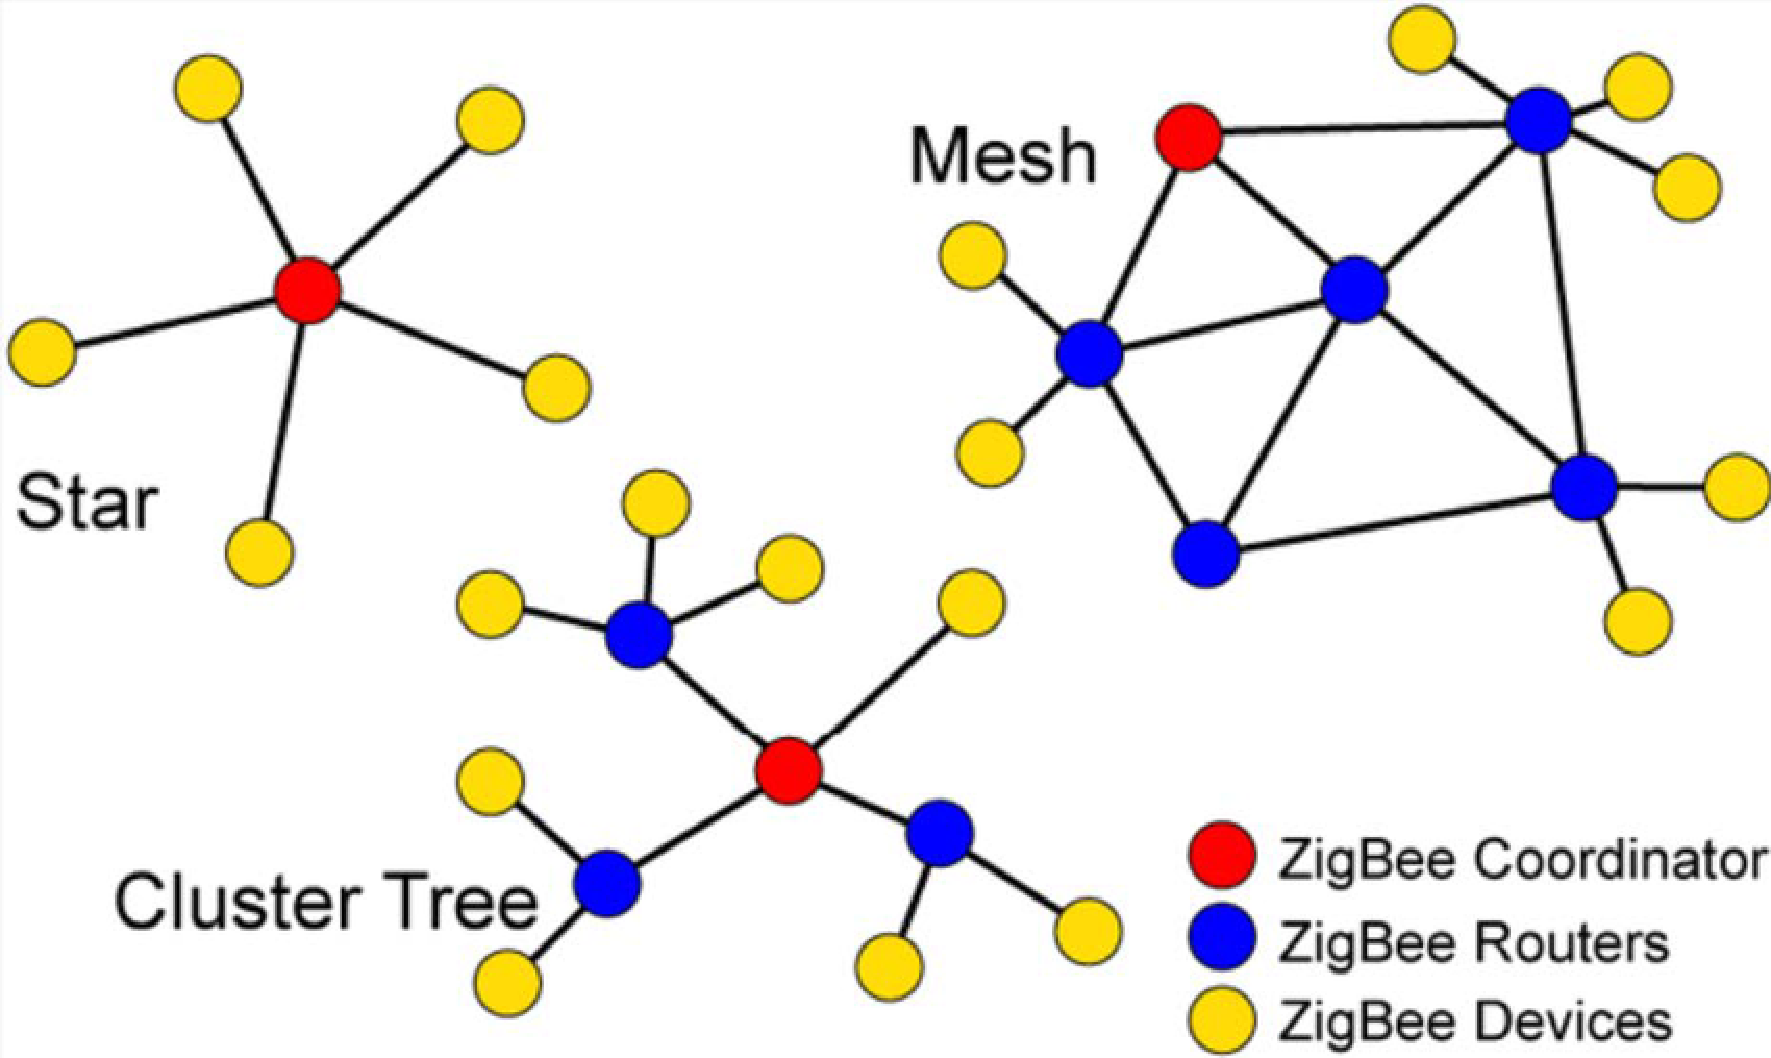
\includegraphics[width=0.5\linewidth]{img/wpan/ztopology}
\end{center}

Si introducono topologie multi-hop, quindi serve avere del routing.

Ci sono due macro classi di nodi: 
\begin{itemize}
	\item \textbf{Full Function Device FFD}
	\item \textbf{Reduced Function Device RFD}
\end{itemize}
Il nome è abbastanza autoesplicativo, tra i FFD c'è un solo coordinatore (ZigBee Coordinator) ed uno o più Router, i quali possono fare instradamento. Gli end device sono (solitamente) RFD, non possono fare routing, possono solo comunicare e ricevere dati verso il coordinatore/loro router di competenza (questi sono sensori, raccolgono dati/piccole azioni).

Quindi i dispositivi possono fare da:
\begin{itemize}
	\item \textbf{Coordinator} (PAN coordinator) FFD: unico all'interno della rete, la crea e ne mantiene le informazioni (es. chiavi di sicurezza)
	\item \textbf{Router} FFD: nodi che hanno la capacità di inoltrare dati tra i dispositivi ZigBee
	\item \textbf{End device} RFD: da punto di vista di rete possiedono solo la funzionalità di parlare ad un router/coordinatore; ridotta complessità ed elevato risparmio energetico
\end{itemize}

\paragraph{Tipologie di invio dati:} Ci sono diverse possibili tipologie di dati, in base al caso d'uso: 
\begin{itemize}
	\item \textbf{Dati periodici}: invio dopo un intervallo di trasmissione fissato (es: sensori per misurare qualcosa)
	\item \textbf{Dati intermittenti (asincroni)}: i dati vengono comunicati in base ad un evento (es: qualsiasi tipo di attuatore come un interruttore)
	\item \textbf{Dati ripetitivi e a bassa latenza}: allocazione di time slot (es: mouse)
\end{itemize}

\paragraph{Architettura:} L'architettura di ZigBee si presenta come:
\begin{center}
	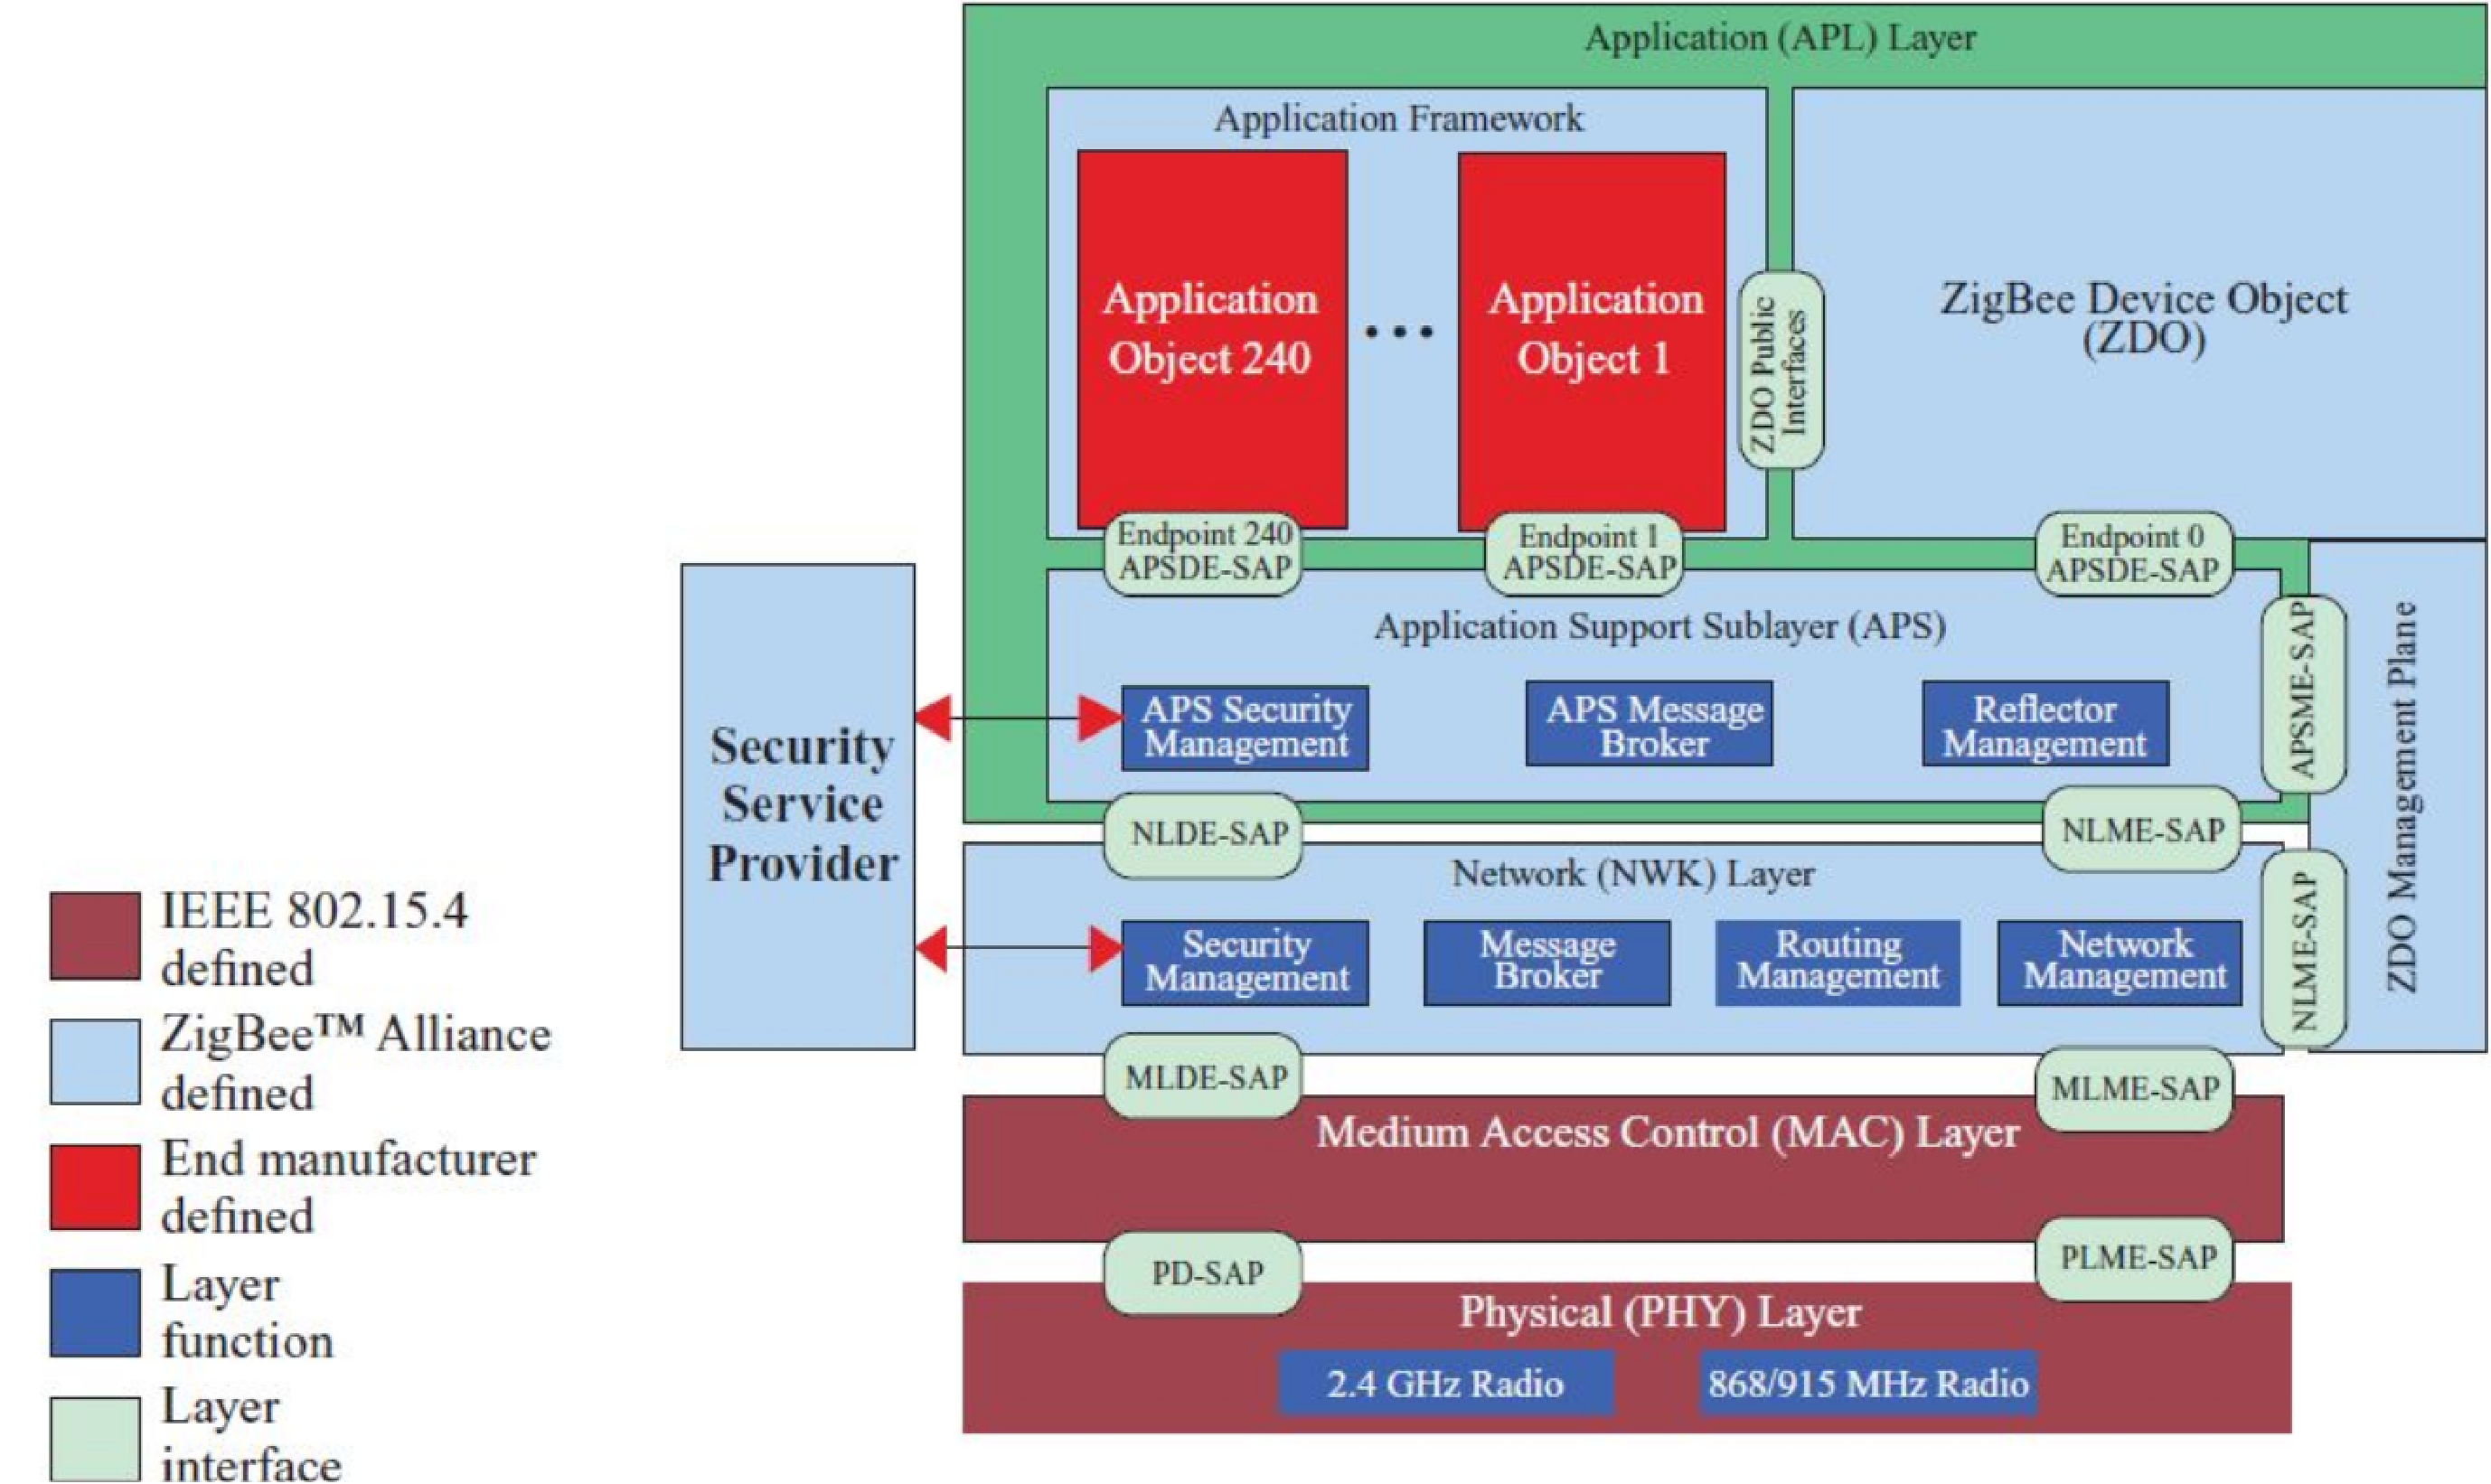
\includegraphics[width=0.98\linewidth]{img/wpan/zarch}
\end{center}

\subsubsection{Livello Fisico 802.15.4 (PHY)}
Lo standard 802.15.4 specifica la tipologia di modulazione e spread spectrum per le 3 bande
\begin{center}
	\renewcommand{\arraystretch}{1.5}
	\resizebox{\textwidth}{!}{  % Resize table to fit page width
		\begin{tabular}{|>{\centering\arraybackslash}p{2.5cm}|>{\centering\arraybackslash}p{1.8cm}|
				>{\centering\arraybackslash}p{2.5cm}|>{\centering\arraybackslash}p{2.5cm}|
				>{\centering\arraybackslash}p{2.5cm}|>{\centering\arraybackslash}p{2.5cm}|
				>{\centering\arraybackslash}p{1.8cm}|}
			\hline
			\textbf{Banda} & \textbf{\# Canali} & \multicolumn{3}{c|}{\textbf{Spread Spectrum}} & \multicolumn{2}{c|}{\textbf{Data rate}} \\ 
			\hline
			& & \textbf{Tipo} & \textbf{Chip Rate (chip/s)} & \textbf{Modulazione (dei chip)} & \textbf{Symbol rate} & \textbf{Bit rate} \\ 
			\hline
			868-868.6 MHz & 1 & DSSS \newline 1bit → 15 chip (max) & 300.000 & BPSK \newline 1 chip & 20 ksym/s & 20 kb/s \\ 
			\hline
			902-928 MHz & 10 & DSSS & 600.000 & BPSK \newline 1 chip & 40 ksym/s & 40 kb/s \\ 
			\hline
			2400-2483.5 MHz & 16 & DSSS \newline 4 → 32 chip \newline (16 sequenze di 32 chip quasi ortogonali) & 2.000.000 & O-QPSK \newline 2 chip & 62.5 ksym/s \newline (1 simbolo di 32 chip → 4 bit) & 250 kb/s \\ 
			\hline
		\end{tabular}
	}
\end{center}

Si usa multiplexing su canali all'interno della banda, spread spectrum DSSS per la comunicazione. Si può notare che i data rate sono molto limitati, ma i dati generalmente trasferiti da sensori/casi d'uso di ZigBee sono anch'essi abbastanza ridotti.

\subsubsection{Livello Data Link 802.15.4 (MAC)}

Questo livello si occupa di:
\begin{itemize}
	\item Gestire l'invio dei beacon (se il dispositivo è PAN Coordinator)
	\item Sincronizzazione con i beacon del coordinatore (router \& end device)
	\item Associazione/dissociazione alla Pan ascoltando i beacon
	\item Accesso al canale tramite CSMA/CA
	\item MAC Address (16 o 64 bit)
	\item Gestione del duty cicle del dispositibo
\end{itemize}

Si possono avere due tipi di trasmissioni: 
\begin{itemize}
	\item diretta: dispositivo $\leftrightarrow$ coordinatore
	\item indiretta: coordinatore $\rightarrow$ dispositivi
\end{itemize}

\paragraph{Modalità di trasferimento:} Ci sono due modalità
\begin{itemize}
	\item \textbf{Unslotted CSMA/CA} senza ausilio di beacon
	\item \textbf{Slotted CSMA/CA utilizzo di beacon}
\end{itemize}

\paragraph{Slotted CSMA/CA:} La modalità slotted si fonda sull'invio di \textbf{beacon}. Questi sono inviati dal coordinatore ed eventualmente inoltrati dai router. Il coordinatore invia periodicamente dei beacon per:
\begin{itemize}
	\item sincronizzare gli altri dispositivi
	\item organizzare i periodi di trasmissione per le diverse tipologie di trasmissione (periodiche, asincrone e bassa latenza)
	\item gestione della trasmissione indiretta: il coordinatore mantiene in una lista le frame non ancora mandate ai dispositivi (poi i dispositivi faranno "Ah devo ricevere qualcosa, ascolterò quello che ha da mandarmi"); nei beacon frame trasmette anche la lista dei dispositivi che hanno frame pendenti (gli dà il permesso di parlare); i dispositivi che ascoltano i beacon sanno se c'è qualcosa per loro
\end{itemize} 

L'organizzazione che il coordinatore ha in mente (solo logica) per la gestione del tempo di comunicazione è definita \textbf{superframe} (sostanzialmente tutto ciò che passa tra un beacon e l'altro).
\begin{center}
	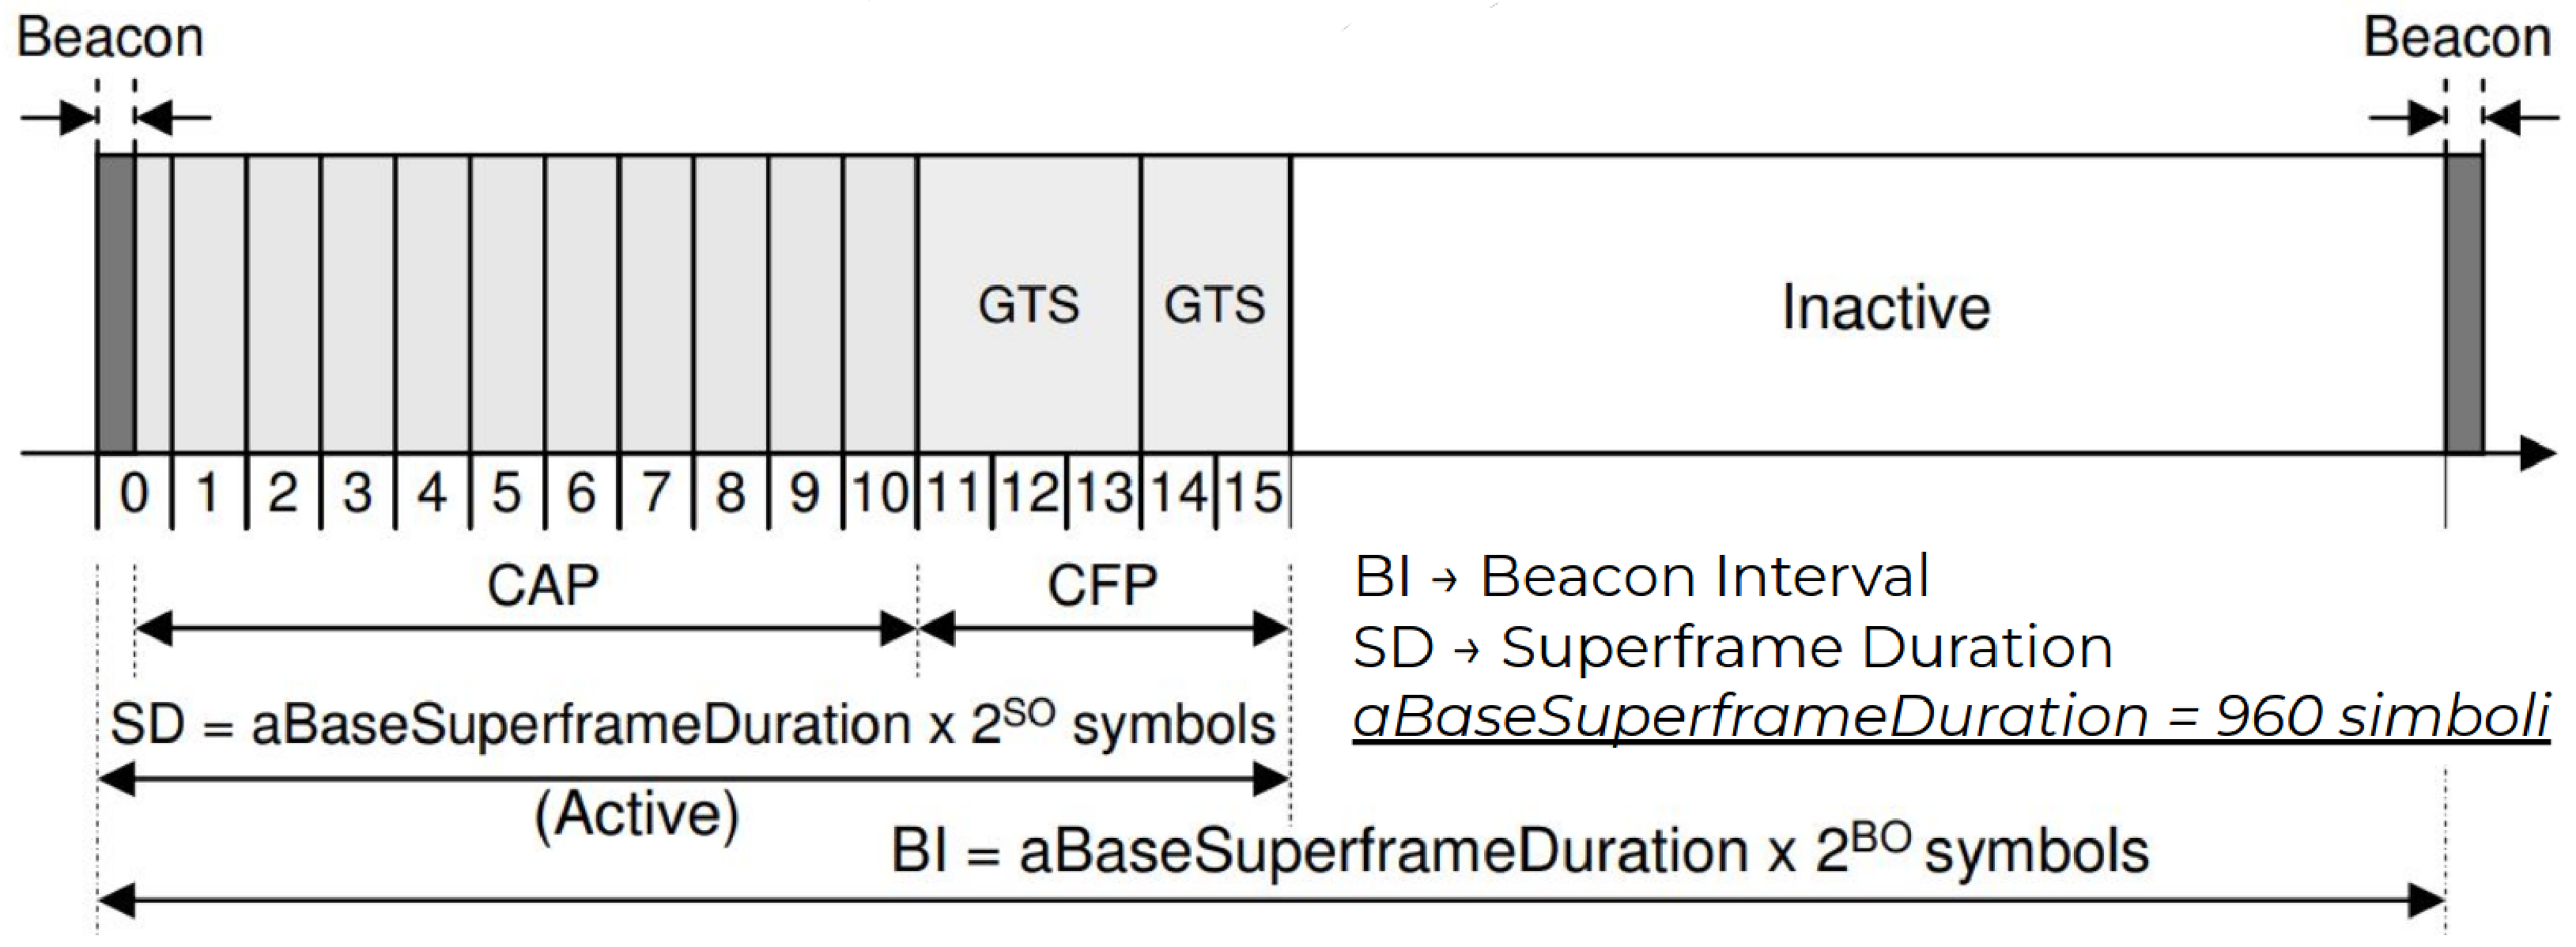
\includegraphics[width=0.98\linewidth]{img/wpan/zsuperframe}
\end{center}
La prima metà è un momento di attività, la seconda è di inattività, poi si ripete il duty cycle. Il \textbf{duty cycle} vuol dire che si alternano periodi di attività, in cui la radio è accesa, a periodi di inattività, a radio spenta (momenti in cui non ci sono trasmissioni programmate, quindi è inutile tenere la radio accesa). Per sincronizzare il duty cycle, all'interno di ogni beacon è presente l'informazione su quando sarà il beacon seguente e questo accenderà la radio appena prima.
Se un dispositivo non deve inviare/ricevere niente, spegne la radio fino al superframe successivo.

Nello standard c'è una $aBaseSuperframeDuration = 960$ $symbols$, quindi ogni beacon avrà una durata multipla di questa unità base. Due parametri che determinano il duty cycle: 
\begin{itemize}
	\item \textbf{Beacon Order BO}: determina il beacon interval 0-14, il quale dura
	$$ BI = aBaseSuperframeDuration \cdot 2^{BO} symbols $$
	\item \textbf{Superframe Order SO}: determina la durata del superframe 0-14: 
	$$ SD = aBaseSuperframeDuration \cdot 2^{SO} symbols $$
\end{itemize}
$960$ simboli sono $\sim 15.3 ms$ in banda $2.4 GHz$. Il duty cycle è dato da 
$$ Duty-Cycle = \frac{2^{SO}}{2^{BO}} $$

Quindi, un sensore, potrebbe accendere la radio per circa $15ms$ per poi spegnere la radio fino alla trasmissione successiva, che potrebbe essere dopo 15 \textit{minuti}. In realtà si riaccende un pochino prima del beacon per tenere conto di una possibile deriva del clock.

\paragraph{Beacon Frame:} Un Beacon Frame è composto da
\begin{center}
	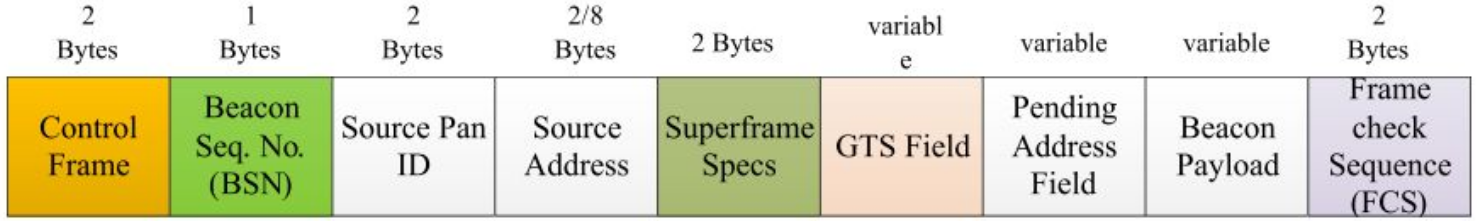
\includegraphics[width=0.95\linewidth]{img/wpan/zbframe}
\end{center}

Il campo Superframe Specs è a sua volta diviso in 
\begin{center}
	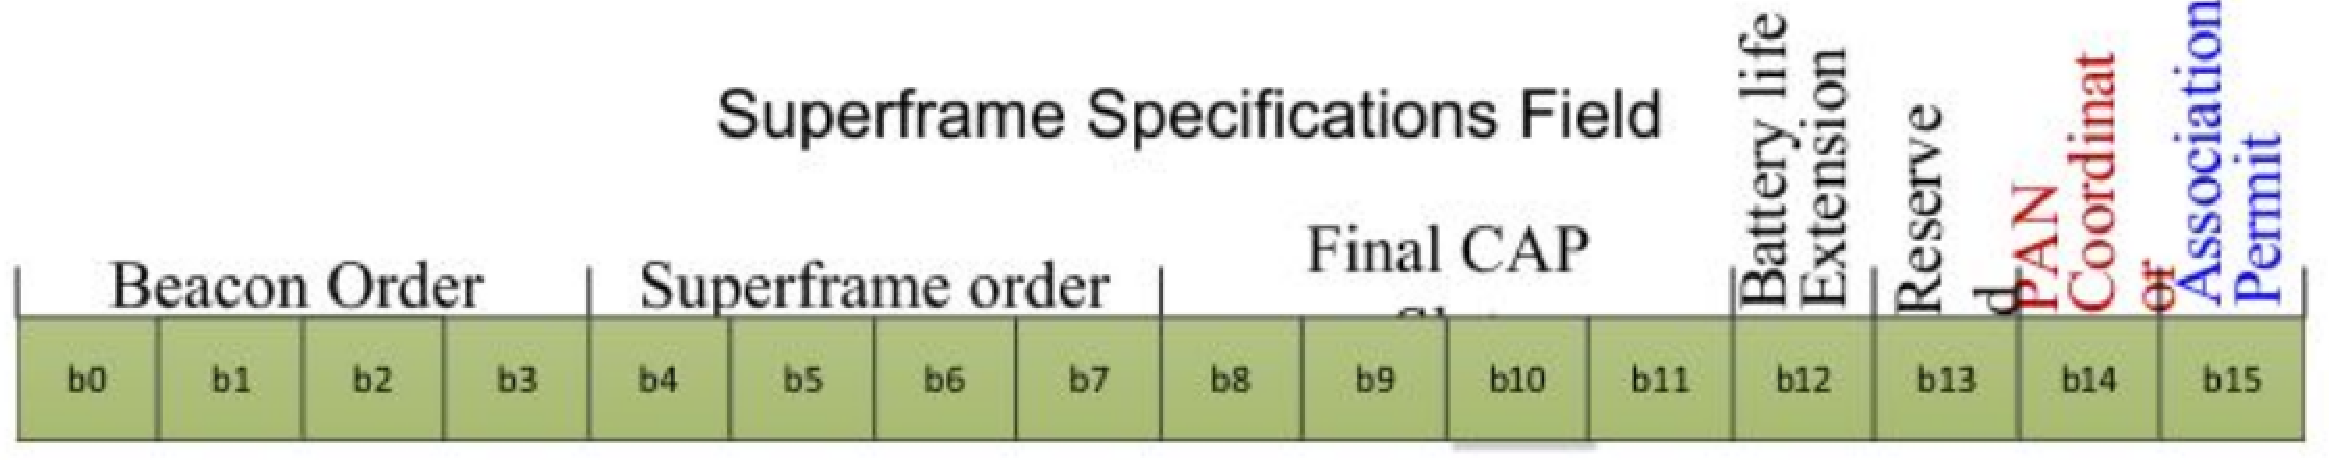
\includegraphics[width=0.75\linewidth]{img/wpan/zssf}
\end{center}

Dove:
\begin{itemize}
	\item Beacon Order: 4 bit per il beacon interval, la frequenza con cui vengono trasmessi i beacon
	\item Superframe Order: 4 bit, definisce la durata della parte attiva del superframe
	\item Final CAP: 4 bit, stabilisce dove termina il periodo CAP all'interno della parte attiva
	\item Battery Life Extension: 1 bit, se a 1 abilita un meccanismo di risparmio energetico
	\item Riservato: 1 bit
	\item PAN Coordinator: 1 bit, indica se chi trasmette il beacon è il coordinatore o un router
	\item Association Permit: 1 bit, indica se altri dispositivi possono associarsi alla rete tramite il dispositivo che trasmette il beacon
\end{itemize}

Gli altri campi all'interno del beacon sono: 
\begin{itemize}
	\item Control Frame: specifica il tipo di frame ed altri parametri relativi alle caratteristiche della trasmissione
	\item Beacon Sequence Number: valore incrementale per identificare il singolo beacon
	\item Source PAN ID: indica l'ID di rete del dispositivo che trasmette il beacon, identifica l'appartenenza del beacon ad una specifica rete
	\item Source Address: Indirizzo del dispositivo che trasmette il beacon
	\item Guaranteed Time Slot (GTS) Field: specifica i time slot riservati per la trasmissione di alcuni dispositivi collision free
	\item Pending Address Field: indica se il coordinatore ha dati in sospeso per uno o più dispositivi
	\item Beacon Payload: può contenere informazioni aggiuntive specifiche del livello di rete ZigBee o altre informazioni proprietarie del produttore
	\item Frame Check Sequence (FCS): campo per il controllo dell'integrità (CRC)
\end{itemize}

Se un dispositivo legge il GTS e il Pending Address e capisce di "non aver nulla da fare", può spegnere la radio fino al prossimo beacon.

Il superframe viene diviso in \textbf{slot con diversi tipi di accesso}:
\begin{itemize}
	\item \textbf{Contention Access Period CAP} (valore di default 16): Accesso al canale usando CSMA/CA
	\item \textbf{Contention Free Period CFP} (da 0 a 7 slot): Intervallo per le comunicazioni con banda riservata tramite Guaranteed Time Slot
\end{itemize}

\paragraph{Slotted CAP CSMA/CA:} Canale a contesa, Carrier Sense Multiple Access con Collision Avoidance. Per capire quando è libero il canale viene fatto un \textbf{Clear Channel Assessment} (CCA) per brevi periodi (8 simboli). Ci sono dei parametri che determinano come questo viene fatto:
\begin{itemize}
	\item $NB=$ Numero di Backoff, inizialmente 0, aumenta di 1 se il canale è occupato
	\item $BE=$ Backoff Exponent, indica il range del periodo di backoff $[0, 2^{BE} - 1]$
	\item $CW=$ Contention Window, indica il numero di slot liberi consecutivi necessari prima di cominciare a trasmettere
\end{itemize}
Ogni contention slot è 20 simboli.

Viene scelto un intero casuale nell'intervallo determinato dal $BE$, si aspetta quel numero di contention slot, e poi vengono fatti $CW$ CCA, se dopo gli assessment il canale è libero il dispositivo comincia a trasmettere. I CCA sono ravvicinati tra loro.

\begin{center}
	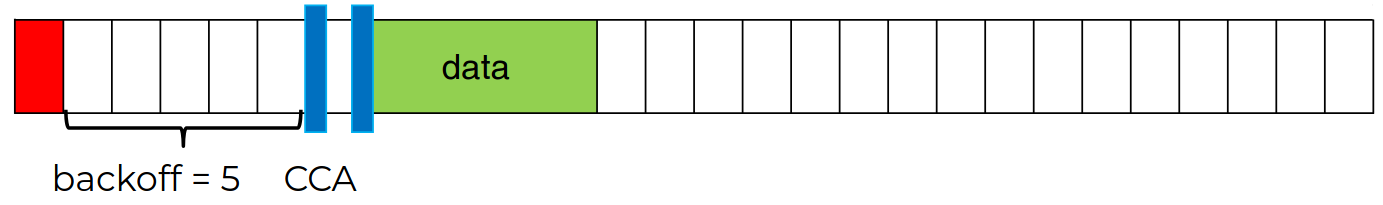
\includegraphics[width=0.9\linewidth]{img/wpan/zex1}
\end{center}

Se durante uno dei CCA viene ricevuta la trasmissione di un altro dispositivo viene allargata la finestra del random backoff ("siamo un po' meglio aspettare per essere sicuri"), incrementando $BE$ e $NB$, prima di fare un altro random backoff e tentativi di CCA. Dopo 4 tentativi ($NB=4$) il livello MAC dichiara transmission failure.

Se il numero di contention slot in CAP non è sufficiente (ho meno slot rispetto al valore casuale che ho estratto), il conteggio viene interrotto e ripreso al superframe successivo (per evitare che un dispositivo sfortunato non trasmetta mai).

In qualsiasi caso, tutta la comunicazione deve terminare prima degli slot GTS, tutto deve essere incluso nel CAP. Se un dispositivo non avrebbe tempo di trasmettere i dati che deve (troppi pochi slot rimanenti), la trasmissione viene rimandata al superframe successivo.

Una trasmissione completa diventa:
\begin{center}
	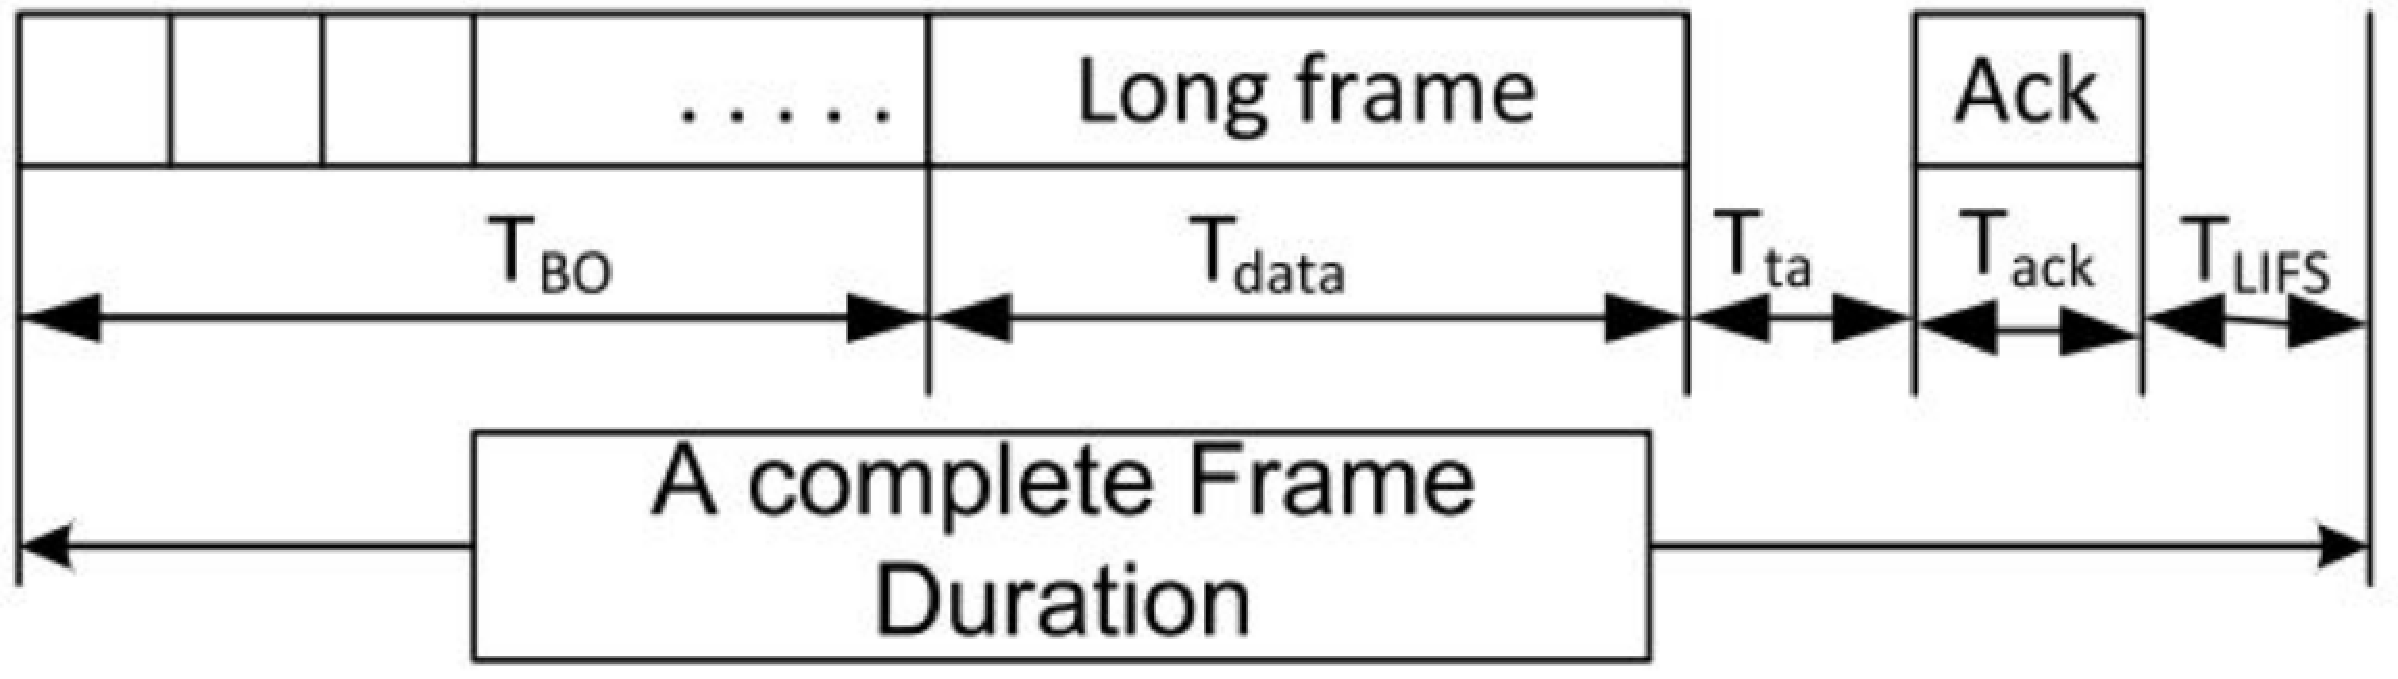
\includegraphics[width=0.7\linewidth]{img/wpan/ztran}
\end{center}
Tempo di backoff $T_{BO}$, un frame di dati $T_{data}$, un tempo di turn around $T_a$ (aspettare che la radio passi da TX a RX), ricezione dell'ack ed un tempo per chiudere la telecomuncazione $T_{LIFS}$ (long inter-frame space).

\paragraph{Unslotted Non Beacon Mode:} Nella modalità senza beacon i dispositivi accedono al canale usando CSMA/CA senza i vincoli di slot. Non c'è sincronizzazione, il tempo è continuo, il controller è più semplice.

Sostanzialmente si ripete la fase di backoff e CSMA/CA finché non il dispositivo non riesce a trasmettere. Non essendoci sincronizzazione, tutto ciò che non è end device deve essere sempre attivo (radio sempre accesa, non sapendo quando qualcuno trasmetterà).

\subsubsection{Livello di rete}
Il livello di rete (Network Layer) di ZigBee (definito nello standard ZigBee, \textbf{sopra} l'IEEE 802.15.4) si occupa della gestione e del mantenimento della topologia di rete e delle operazioni di routing. 

In particolare, gestisce formazione della rete, indirizzamento sopra al MAC e la topologia (supportando la riconfigurazione). Dato che ci sono trasmissioni che devono giungere a dispositivi non in connessione diretta è necessario routing, questo viene gestito a livello di rete tramite protocolli di routing mesh come \href{https://en.wikipedia.org/wiki/Ad_hoc_On-Demand_Distance_Vector_Routing}{\texttt{Ad-Hoc On Demand Distance Vector AODV}}.

\subsubsection{ZigBee Device Object ZDO}
Posizionato sopra il livello di rete, definito nello standard ZigBee. Definisce il \textbf{ruolo del dispositivo}, permette la scoperta di nuovi dispositivi e le loro funzionalità. Inoltre fornisce un'interfaccia comune per le applicazioni.

Stabilisce come un dispositivo si inserisce nella rete, come scopre gli altri nodi e come gestisce la sicurezza e le funzionalità di base. Ogni nodo ZigBee ha il proprio ZDO che fornisce servizi di gestione e supervisione, rendendo possibile l’interoperabilità fra dispositivi di diversi produttori. 

\subsection{Matter \& Thread}
%Maybe img s32
Thread ha il livello fisico e MAC secondo standard 802.15.4, ma sopra usa uno stack
\begin{center}
	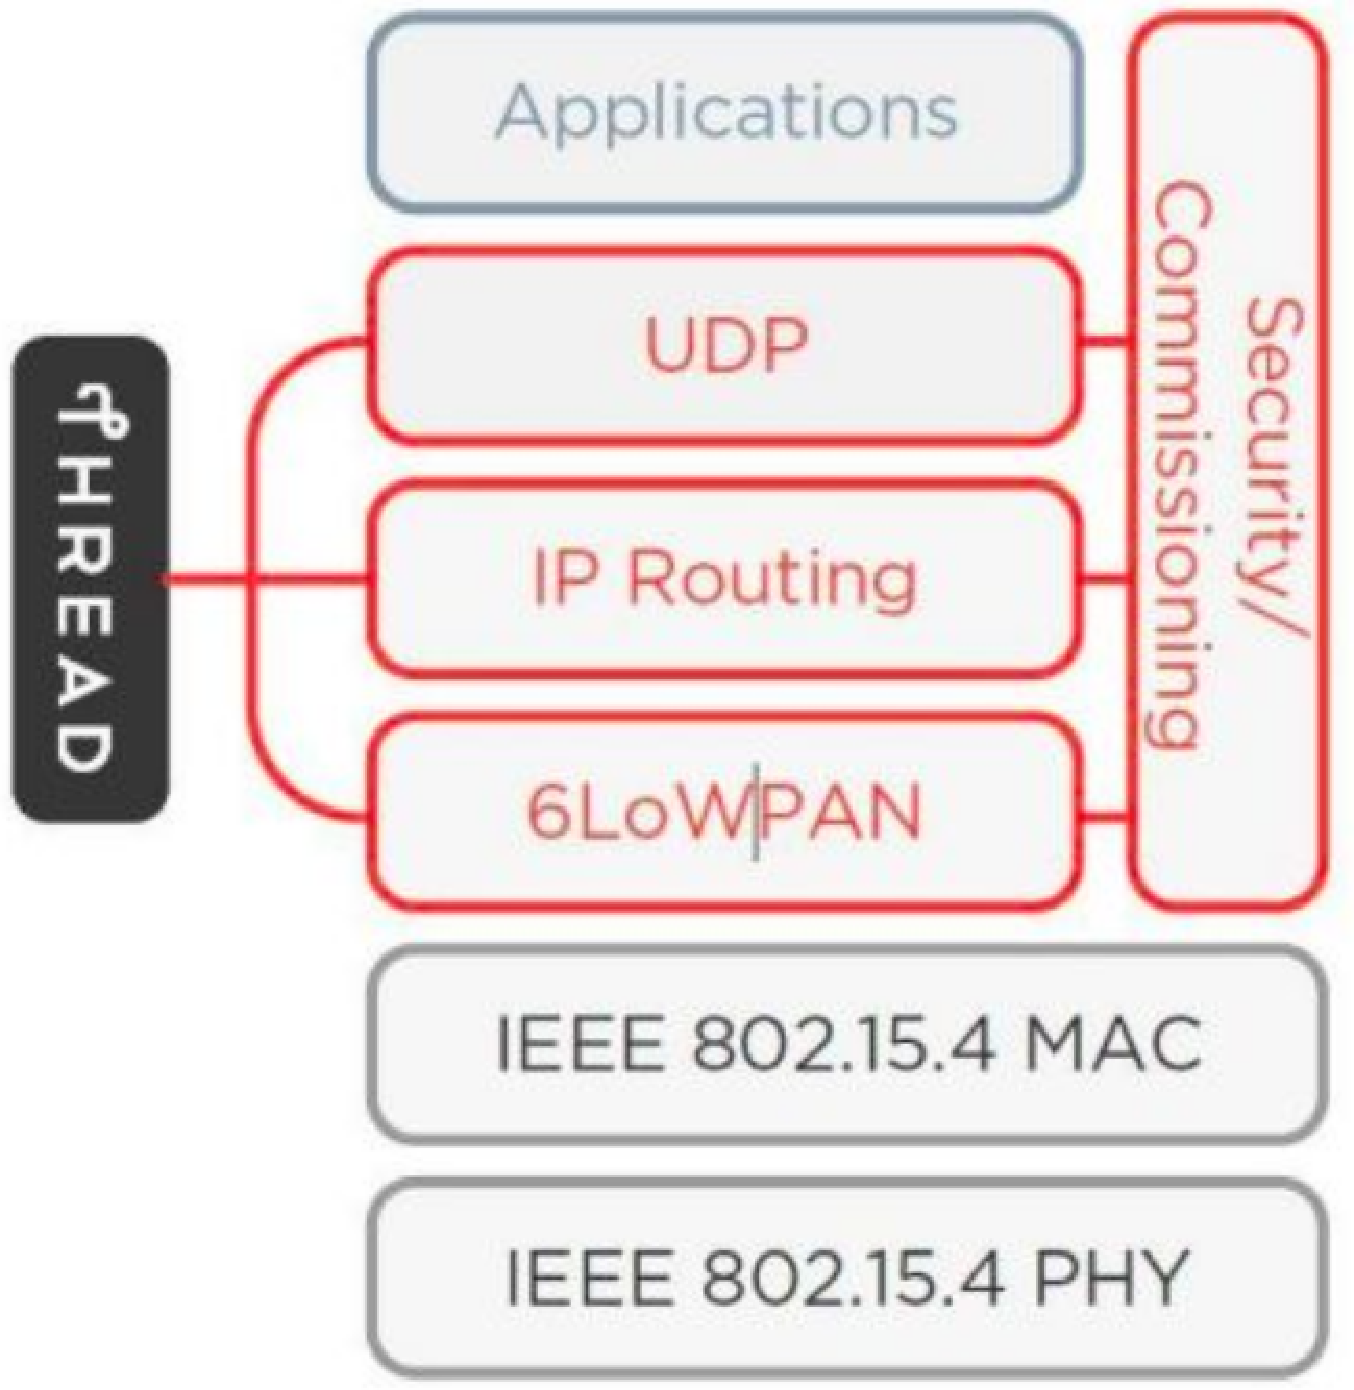
\includegraphics[width=0.5\linewidth]{img/wpan/thread}
\end{center}
\begin{itemize}
	\item Standard 6LoWPAN, compressione header, supporto a rete mesh
	\item IP Routing, indirizzamento IPv6, distance vector routing, costi dei link variabili in base a RSSI (Received Signal Strength Indicator)
	\item UDP
\end{itemize}

\paragraph{Rete Thread:} Cambiano un po' le capacità dei dispositivi, ci sono: 
\begin{itemize}
	\item \textbf{Routing Full Thread Device}: possono essere
	\begin{itemize}
		\item \textbf{router}: effettua routing e fornisce servizi di accesso e sicurezza (NoSleep, può essere "degradato" a Router-Eligible End Device REED)
		\item \textbf{leader}: un router con funzionalità aggiuntive che può eleggere/destituire REED
	\end{itemize}
	\item \textbf{Non routing Full Thread Device}: si dividono in
	\begin{itemize}
		\item REED
		\item Full End Device FED, non possono essere eletti router
	\end{itemize}
\end{itemize}

I Non Routing Minimal Thread Devices sono dispositivi con requisiti HW minori:
\begin{itemize}
	\item Minimal End Device (MED): comunica solo con il router genitore e radio sempre attiva
	\item Sleepy End Device (SED): comunica solo con il router genitore e duty-cycle
	\item Synchronized Sleepy End Device (SSED): comunica solo con il router genitore e duty-cycle secondo intervalli schedulati
\end{itemize}

\paragraph{Border router:} Sono dei dispositivi di tipo Full Thread Device che forniscono connettività verso le altre reti con un livello fisico diverso (Wi-Fi, Ethernet, \dots). Offre funzionalità di routing all'esterno della rete thread.

%Fine S3

%Fine PAN